\documentclass[10pt,a4paper,final,oneside,openany]{memoir}

\input{defaultprelude.tex}

\usepackage[titelside, en, nat]{ku-forside}

\titel{Exploiting functional invariants}
\undertitel{to optimise parallelism: a dataflow approach}
\forfatter{Troels Henriksen -- \texttt{athas@sigkill.dk}}
\forfatterET{}
\forfatterTO{}
\opgave{Master's Thesis} % Findes kun under 'titelside'
\dato{February 2014}
\vejleder{Supervisors: Cosmin Eugen Oancea and Fritz Henglein}

\newcommand\boolt[0]{\texttt{bool}}
\newcommand\realt[0]{\texttt{real}}
\newcommand\chart[0]{\texttt{char}}
\newcommand\intt[0]{\texttt{int}}
\newcommand\aliases[1]{\textrm{aliases}(#1)}
\renewcommand\tilde[0]{{\raise.17ex\hbox{$\scriptstyle\sim$}}}
\newcommand{\LO}{$\mathcal{L}_0$}

\newcommand{\tagsc}[1]{\tag{\textsc{#1}}} % Fake Small Caps tagging
\newcommand{\nfrac}[2]{\frac{\displaystyle{#1}}{\displaystyle{#2}}}
\newcommand*{\bfrac}[2]{\genfrac{}{}{0pt}{}{#1}{#2}}

\definecolor{DikuRed}{RGB}{130,50,32}
\newcommand{\emp}[1]{\textcolor{DikuRed}{ #1}}
\definecolor{CosGreen}{RGB}{10,100,70}
\newcommand{\emphh}[1]{\textcolor{CosGreen}{ #1}}

\newcommand{\mymath}[1]{$ #1 $}
\newcommand{\myindx}[1]{_{#1}}
\newcommand{\myindu}[1]{^{#1}}
\newcommand{\mymathbb}[1]{\mathbb{#1}}
\newcommand{\cindx}[1]{\(\myindx{#1}\)}

% Write "Part II" etc. in TOC instead of just "II"
\renewcommand*{\cftpartname}{Part\space}

\bibliography{bibliography}

\begin{document}
\frontmatter

 \clearpage

\maketitle
~
\vspace{3cm}
  \begin{abstract}
    We present a pure functional data-parallel programming language
    supporting nested parallelism on regular data.  Our language is
    aimed at execution on massively parallel SIMD hardware, such as
    modern graphics-programming units.  The language contains novel
    features for performing in-place modification of arrays without
    violating functional purity.

    Furthermore, our language includes an assertion system that can be
    used to express dynamic checks such as bounds checks directly in
    the language, potentially facilitating their removal from inner
    loops through standard optimisations.

    We discuss the design and implementation of several optimisations,
    notably an advanced hoister, and loop fusion based on a structural
    transformation, which is capable of fusing operations where the
    output is used in multiple places, when possible without
    duplicating computation.  This is an unusual feature among fusion
    transformations.

    The benefit of our optimisations are demonstrated on three
    real-world benchmarks translated to our programming language.  We
    argue that always refusing to duplicate computation is too
    conservative on parallel hardware, and discuss potential
    directions for further improvement.
  \end{abstract}

% \clearpage
%  ~\thispagestyle{empty}
\clearpage
\tableofcontents*
%\openany
\phantomsection
\addcontentsline{toc}{chapter}{Preface}
\chapter*{Preface}
This dissertation is submitted in fulfillment of the graduate education
in computer science (\textit{Datalogi}) at the University of
Copenhagen, for Troels Henriksen.
%\openright
\mainmatter
\counterwithout{table}{chapter}
\counterwithout{figure}{chapter}
\chapter{Introduction}

For practically the entire lifetime of the electronic computer,
programmers have been used to an exponential growth in commonly
available computing power.  Until around 2006, this directly
manifested itself as improvements to sequential performance, although
physical limits made it uneconomical (or impossible) for this trend to
continue.  These days, hardware designers are making their machines
increasingly \textit{parallel}: rather than speeding up the individual
processors, as happened previously, \textit{more} processors, or more
\textit{specialised} processors, are added.  Thus, while computing
power is still growing, it has become increasingly necessary to write
programs that are parallel in order to take full advantage of modern
hardware.

One interesting development is the commoditisation of massively
parallel vector processors in the form of graphics cards.  While
hardware acceleration of graphics became commonplace in the 90s, it
was not until the rise of CUDA and OpenCL in 2006 that
\textit{General-Purpose computing on Graphics Processing Units}
(GPGPU) began to move into the mainstream.

... \fxnote{Insert more - convince reader that my work addresses an
  important problem, and that I will give a well thought-out solution.
  Why is \LO{} functional, and why does it support sequential loops
  anyway?}

Throughout this thesis, we will often refer to a vaguely defined
``programmer'', as well as ascribe various motives and expectations to
this nebulous being.  While \LO{} is intended as an intermediate
language, and in the end is intended as a target language by compilers
for higher-level languages, it has a well-defined human-readable (and
writable) syntax, and can be programmed directly.  Indeed, all extant
\LO{} programs have been written by hand.  Thus, when ``the
programmer'' is referenced, we can refer to either an actual human, or
a compiler generating \LO{} code.  For our purposes, these will have
identical motives, although a human programmer may complain somewhat
more vocally about the lack of syntactical niceties in the language.

\section{Contributions}

We present a purely functional data-parallel programming language,
\LO{}, supporting nested parallelism.  The language supports a method
\fixme{Why do I support nested parallelism?  Why only regular arrays?
  Why are in-place updates supported (cross-iteration dependent
  loops)} for safely performing in-place updates of array data through
a type system concept called \textit{uniqueness types}.  Through the
translation of real-world financial programs to \LO{}, we demonstrate
the practical usefulness of this language feature.

We present the design and implementation of several optimisations,
notably hoisting bounds checks out of inner loops, and loop fusion
based on a structural transformation.  The fusion transformation is
capable of fusing loops whose output is used in multiple places, when
possible without duplicating computation.\fixme{Why is it important to
  hoist bounds checks?  Because we target aggressive (static+dynamic)
  analysis; this is an instance of optimising arbitrary predicates.}

The benefits of our optimisations are demonstrated on three real-world
financial benchmarks.  It is shown that the compiler is able to hoist
bounds checks and other assertions outside of loops.

The effectiveness of fusion is demonstrated via compiler
instrumentation and quantitative and qualitative measurements on the
three benchmarks, in the form of inspecting the changes in program
dataflow.  This shows that always refusing to duplicate computation is
too conservative on parallel hardware, and discuss potential
directions for further improvement.

The implementation of the \LO{} compiler consists of roughly ten
thousand lines of Haskell (ignoring comments and blank lines), and it
is hosted and publicly browsable at
\url{https://github.com/HIPERFIT/L0Language}.

Parts of this thesis, in particular the core of the fusion algorithm
in \cref{chap:fusion}, has been previously published as

\begin{quote}
\fullcite{Henriksen:2013:TGA:2502323.2502328}
\end{quote}

\section{Report outline}

The remainder of the report is structured as follows.
\Cref{chap:l0language,chap:uniqueness-types} will introduce the
programmer-visible part of \LO{} and serves as a language reference.
\Cref{chap:internal} presents a slight modification of the external
language, that makes it more amenable to transformation and
optimisation.  \Cref{chap:first-order-optimisations} discusses various
classical optimisations in the context of \LO{}.  \Cref{chap:fusion}
covers \textit{loop fusion}, an important optimisation, while
\cref{chap:fusion-enabling-soac-transformations,chap:hindrance-removal}
cover transformations that enable other optimisations (although
particularly fusion).

\section{Notation}

In various places, I will use an \(\overline{\text{overline}}\) to
indicate a comma-separated sequence of terms.  For example, when
describing a function call, rather than writing:
\[
f(e_{1},\ldots,e_{n})
\]
I may instead write:
\[
f(\overline{es})
\]
I may also use this in conjunction with expliclt arguments, as in:
\[
f(e_{start},\overline{es},e_{end})
\]

%%% Local Variables:
%%% mode: latex
%%% TeX-master: "thesis"
%%% End:


\part{Language Design}
\label{part:languagedesign}

\chapter{The \LO{} language}

\section{First-order \L0{}}

\begin{figure}[bt]
\begin{tabular}{lrll}
$t$ & $::=$ & \texttt{int} & (Integers) \\
& $|$ & \texttt{real} & (Floats) \\
& $|$ & \texttt{bool} & (Booleans) \\
& $|$ & \texttt{char} & (Characters) \\
& $|$ & \texttt{\{$t_{1}$, \ldots, $t_{n}$\}} & (Tuples) \\
& $|$ & \texttt{[$t$]} & (Arrays) \\
& $|$ & \texttt{*[$t$]} & (Unique arrays) \\
\\
$v$ & $::=$ & $k$ & (Integer)\\
& $|$ & $x$ & (Decimal number) \\
& $|$ & $b$ & (Boolean)\\
& $|$ & $c$ & (Character)\\
& $|$ & $\{v_{1},\ldots,v_{n}\}$ & (Tuple) \\
& $|$ & $[v_{1},\ldots,v_{n}]$ & (Array) \\
\\
$p$ & $::=$ & \texttt{\textbf{id}} & (Name pattern)\\
& $|$ & \texttt{($p_{1}$, \ldots, $p_{n}$)} & (Tuple pattern) \\
\\
$e$ & $::=$ & $v$ & (Constant)\\
& $|$ & $\textbf{id}$ & (Variable)\\
& $|$ & \texttt{($e_{1}$,\ldots,$e_{n}$)} & (Tuple expression) \\
& $|$ & \texttt{\{$e_{1}$,\ldots,$e_{n}$\}} & (Array expression) \\
& $|$ & $e_{1} \odot{} e_{2}$ & (Binary operator) \\
& $|$ & \texttt{\tilde{} $e$} & (Prefix minus) \\
& $|$ & \texttt{not $e$} & (Logical negation) \\
& $|$ & \texttt{if $e_{1}$ then $e_{2}$ else $e_{3}$} & (Branching) \\
& $|$ & \texttt{\textbf{id}[$e_{1}$, \ldots, $e_{n}$]} & (Indexing) \\
& $|$ & \texttt{\textbf{id}($e_{1}$, \ldots, $e_{n}$)} & (Function call) \\
& $|$ & \texttt{let $p$ = $e_{1}$ in $e_{2}$} & (Pattern binding) \\
& $|$ & \texttt{zip($e_{1}$, \ldots, $e_{n}$)} & (Zipping) \\
& $|$ & \texttt{unzip($e$)} & (Unzipping) \\
& $|$ & \texttt{iota($e$)} & (Range) \\
& $|$ & \texttt{replicate($e_{n}$, $e_{v}$)} & (Replication) \\
& $|$ & \texttt{size($e$)} & (Array length) \\
& $|$ & \texttt{reshape(($k_{1}$,\ldots,$k_{n}$), $e$)} & (Array reshape) \\
& $|$ & \texttt{transpose($e$)} & (Transposition) \\
& $|$ & \texttt{split($e_{1}$, $e_{2}$)} & (Split $e_{2}$ at index $e_{1}$) \\
& $|$ & \texttt{concat($e_{1}$, $e_{2}$)} & (Concatenation) \\
& $|$ & \texttt{let $\alpha$ = $\beta$ with} & (In-place update) \\
&     & \texttt{\ \ [$e_{1}$,\ldots,$e_{n}$] <- $e_{v}$} \\
&     & \texttt{in $e_{b}$} \\
& $|$ & \texttt{loop ($p$ = $e_{1}$) =} & (Loop) \\
&     & \texttt{\ \ for $\alpha$ < $e_{2}$ do $e_{3}$} \\
&     & \texttt{in $e_{4}$} \\
\end{tabular}
\\
\begin{tabular}{lrll}
$fun$ & $::=$ & \texttt{fun $t$ \textbf{id}($t_{1}$ \textbf{id}$_{1}$,\ldots $t_{n}$ \textbf{id}$_{n}$) = $e$} \\
\\
$prog$ & $::=$ & $\epsilon$ \\
       & $|$   & $fun$ $prog$
\end{tabular}
\caption{\LO{} syntax}
\label{fig:fo-syntax}
\end{figure}

\section{SOACs}

\begin{figure}[bt]
\begin{tabular}{lrll}
$l$ & $::=$ & \texttt{fn $t$ ($t_{1}$ \textbf{id}$_{1}$, \ldots, $t_{n}$ \textbf{id}$_{n}$)} & (Anonymous function) \\
&     & \texttt{=> $e$} \\
& $|$ & \texttt{\textbf{id} ($e_{1}$, \ldots, $e_{n}$)} & (Curried function) \\
& $|$ & \texttt{op $\odot$ ($e_{1}$, \ldots, $e_{n}$)} & (Curried operator) \\
\\
$e$ & $::=$ & \texttt{map($l$, $e$)} \\
    & $|$ & \texttt{filter($l$, $e$)} \\
    & $|$ & \texttt{reduce($l$, $x$, $e$)} \\
    & $|$ & \texttt{scan($l$, $x$, $e$)} \\
    & $|$ & \texttt{redomap($l_{r}$, $l_{m}$, $x$, $e$)} \\
\end{tabular}
\caption{Second-order array combinators}
\label{fig:soacs}
\end{figure}

\section{Internal constructs}

\begin{figure}[bt]
\begin{tabular}{lrll}
$e$ & $::=$ & \texttt{map2($l$, $e_{1}$, \ldots, $e_{n}$)} \\
    & $|$ & \texttt{filter2($l$, $e_{1}$, \ldots, $e_{n}$)} \\
    & $|$ & \texttt{reduce2($l$, $x_{1}$, \ldots, $x_{n}$, $e_{1}$, \ldots, $e_{n}$)} \\
    & $|$ & \texttt{scan2($l$, $x_{1}$, \ldots, $x_{n}$, $e_{1}$, \ldots, $e_{n}$)} \\
    & $|$ & \texttt{redomap2($l_{r}$, $l_{m}$, $x_{1}$, \ldots, $x_{n}$, $e_{1}$, \ldots, $e_{n}$)} \\
\end{tabular}
\caption{Second-order tuple-array combinators}
\label{fig:tuple-soacs}
\end{figure}

\begin{figure}[bt]
\begin{tabular}{lrll}
$t$ & $::=$ & \texttt{cert} \\
\\
$c$ & $::=$ & \textbf{id}$_1$, \ldots ,\textbf{id}$_{n}$ \\
\\
$e$ & $::=$ & \texttt{assert($e$)} & (Assertion) \\
& $|$ & \texttt{conjoin($e_{1}$, \ldots, $e_{n}$)} & (Conjoin assertions) \\
& $|$ & \texttt{<$c$>\textbf{id}[$e_{1}$, \ldots, $e_{n}$]} & (Indexing) \\
& $|$ & \texttt{<$c$>size($k$, $e$)} & (Array length) \\
& $|$ & \texttt{<$c$>reshape(($k_{1}$,\ldots,$k_{n}$), $e$)} & (Array reshape) \\
& $|$ & \texttt{<$c$>transpose($e$)} & (Transposition) \\
& $|$ & \texttt{<$c$>split($e_{1}$, $e_{2}$)} & (Split $e_{2}$ at index $e_{1}$) \\
& $|$ & \texttt{<$c$>concat($e_{1}$, $e_{2}$)} & (Concatenation) \\
& $|$ & \texttt{let <$c$>$\alpha$ = $\beta$ with} & (In-place update) \\
&     & \texttt{\ \ [$e_{1}$,\ldots,$e_{n}$] <- $e_{v}$} \\
&     & \texttt{in $e_{b}$} \\
\end{tabular}
\caption{Assertions}
\label{fig:assertions}
\end{figure}

%%% Local Variables: 
%%% mode: latex
%%% TeX-master: "thesis.tex"
%%% End: 


\chapter{Uniqueness types}
\label{chap:uniqueness-types}


\chapter{Internal representation}
\label{chap:internal}

It is a common compilation technique to transform the externally
visible language into a simpler intermediate language, on which all
optimisation and further compilation is performed.  This is usually
necessary, because languages written for human consumption have a
large amount of bells and whistles that make programming more
convenient, but offer no significant avenues for optimisation, but
rather just leave more cases for the optimiser to handle.

We do not suffer as badly from that problem with \LO{}, as it was
designed as an intermediate language itself.  Nevertheless, before
embarking on any optimisation, we do transform the input program to an
internal dialect of \LO{}.  In most compilers, it is usually not
possible to transform the intermediate language to the external
language, at least not without losing much of the structure of the
original program.  In comparison, the transformation from external to
internal \LO{} is comparatively simple and reversible (with some loss
of information; see \cref{sec:internal-to-external}).

A very important first notice: All names in internal \LO{} are
\textit{globally unique}.  This means that we will never have name
shadowing, and we can uniquely identify, say, a \texttt{let}-binding
by one of the names it binds.

\section{Tuple transformation}
\label{sec:tuple-transformation}

The principal difference between external and internal \LO{} is the
total absence of arrays of tuples in the latter.  There are several
reasons for this - \cref{chap:fusion} will describe how this benefits
the fusion algorithm, and when generating the final machine code, we
will also not be able to conveniently represent arrays of tuples in
memory.

An array of tuples type is converted to a tuple containing arrays of
the original tuple components, for which the process is then repeated
recursively.  Futhermore, tuples are flattened.  All other types are
left unchanged.  A few examples:

\begin{align*}
\texttt{[int]} &\Rightarrow \texttt{[int]} \\
\texttt{[\{int,real\}]} &\Rightarrow \texttt{\{[int],[real]\}} \\
\texttt{[\{[int], real\}]} &\Rightarrow \texttt{\{[[int]], [real]\}} \\
\texttt{\{\{int, bool\}, real\}} &\Rightarrow \texttt{\{int, bool, real\}} & \text{(Flattening)} \\
\end{align*}

\texttt{zip} and \texttt{unzip} are not allowed in internal \LO{}.
Both are removed during the conversion process, as they perform a
transformation between representations that is not necessary in
internal \LO{}, although \texttt{zip} has some additional
complications that are discussed in \cref{sec:assertions}.

Most expressions operating on arrays of tuples have to be modified to
operate on the components of the replacement tuples-of-arrays instead,
but the transformation is relatively trivial, so we will not describe
it in detail.

Internal \LO{} also does not permit tuple-typed variables.  Hence,
every pattern that binds a variable to a tuple must be converted to
explicitly name the elements of the tuple, e.g:

\begin{colorcode}
let x = \{f(a), g(b)\} in
...
  \(\emp{\Downarrow}\)
let \{x1,x2\} = \{f(a), g(b)\} in
...
\end{colorcode}

\subsection{Tupleless SOACs}

As internal \LO{} does not permit tuples of arrays, we need to find a
way to convert an expression such as:
\begin{colorcode}
map(fn int ({int,int} t) =>
      let {x,y} = t in
      f(x,y),
    zip(a, b))
\end{colorcode}
The solution is tupleless SOACs: variants of the normal SOACs in which
several arrays are traversed in parallel.  For example, the previous
expression will be converted to:
\begin{colorcode}
mapT(fn \{int\} (int x, int y) =>
       f(x,y),
     a, b)
\end{colorcode}
Conceptually, we can imagine that the tuple-SOACs all have a built-in
\texttt{zip}.  Furthermore, initial values for tuple-typed
accumulators (for \texttt{reduceT}, \texttt{scanT} and
\texttt{redomapT}) are given element-wise, and also passed
element-wise to the function.  This, combined with the ban on arrays
of tuples, implies that no parameter of a function in a tupleless SOAC
is ever tuple-typed.

\begin{figure}[bt]
\begin{tabular}{lrll}
$e$ & $::=$ & \texttt{<$c$>mapT(fn $t$ ($t_{1}$ $v_{1}$, \ldots, $t_{n}$ $v_{n}$) => $e_f$, $e_{1}$, \ldots, $e_{n}$)} \\
    & $|$ & \texttt{<$c$>filterT(fn $t$ ($t_{1}$ $v_{1}$, \ldots, $t_{n}$ $v_{n}$) => $e_f$, $e_{1}$, \ldots, $e_{n}$)} \\
    & $|$ & \texttt{<$c$>reduceT(fn $t$ ($t_{1}$ $v_{1}$, \ldots, $t_{n}$ $v_{n}$) => $e_f$, \{$x_{1}$, \ldots, $x_{n}$\}, $e_{1}$, \ldots, $e_{n}$)} \\
    & $|$ & \texttt{<$c$>scanT(fn $t$ ($t_{1}$ $v_{1}$, \ldots, $t_{n}$ $v_{n}$) => $e_f$, \{$x_{1}$, \ldots, $x_{n}$\}, $e_{1}$, \ldots, $e_{n}$)} \\
    & $|$ & \texttt{<$c$>redomapT(fn $t_{o}$ ($t_{o_{1}}$ $v_{o_{1}}$, \ldots, $t_{o_{n}}$ $v_{o_{n}}$) => $e_o$,} \\
    &     & \texttt{\ \ \ \ \ \ \ \ \ \ \ \ fn $t_{i}$ ($t_{i_{1}}$ $v_{i_{1}}$, \ldots, $t_{i_{n}}$ $v_{i_{n}}$) => $e_i$,} \\
    &     & \texttt{\ \ \ \ \ \ \ \ \ \ \ \ \{$x_{1}$, \ldots, $x_{n}$\}, $e_{1}$, \ldots, $e_{n}$)} \\
\end{tabular}
\caption{Tupleless Second-order array combinators}
\label{fig:tupleless-soacs}
\end{figure}

As a minor detail, curried functions are also not permitted in
tupleless SOACs, although we will still use them for notational
convenience.  The notation is summarised on \cref{fig:tupleless-soacs}
- the \texttt{<$c$>} notation is explained in the next section.

\section{Assertions}
\label{sec:assertions}

Removal of \texttt{zip} carries with it an additional complication.
Recall that \texttt{zip} is responsible for checking that the input
arrays are of the same (outer) size, and if they are not, terminate
the program with an error.  The obvious solution is to make each
tupleless SOAC do the same check, but that would be wasteful of
computer resources.  Even worse, it's not a full solution to the
problem.  Consider the following expression.
\begin{colorcode}
let c = zip(a,b) in
c[0]
\end{colorcode}
How should this be transformed?  There is an obvious solution:
\begin{colorcode}
\{a[0], b[0]\}
\end{colorcode}
But it is of course wrong - there is no checking that \texttt{a} and
\texttt{b} are of the same length, hence the original expression may
fail, while the transformed expression may evaluate successfully.  The
final solution is to \textit{predicate} the expression on the fact
that \texttt{a} and \texttt{b} must match.
\begin{colorcode}
if \textit{\texttt{a} and \texttt{b} have the same length}
then \{a[0], b[0]\}
else \textit{fail}
\end{colorcode}
Using branches to accomplish this somewhat complicates further
transformation and optimisation however, so an approach based on
\textit{assertions} was chosen.  First, we introduce a new type,
\texttt{cert}, which is inhabited by only one value \texttt{Checked}.
The idea is that a value of type \texttt{cert} acts as a
\textit{certificate}, certifying that some property has been checked.
We then add three new language constructs:

\begin{description}
\item[\texttt{assert($e$)}]\hfill\\
  Returns \texttt{Checked} if the boolean expression $e$ returns
  \texttt{True}, otherwise terminates the program with an error.

\item[\texttt{conjoin($e_{1}, \ldots, e_{n}$)}]\hfill\\
  All of $e_{1}, \ldots, e_{n}$ must be expressions of type
  \texttt{cert}.  Always returns \texttt{Checked}.  The purpose of
  \texttt{conjoin} is to combine several \texttt{cert} values into
  one.

\item[\texttt{<$v_{1},\ldots,v_{n}$>$e$}]\hfill\\
  A predicated expression.  Evaluate $e$ and return its value.  The
  variables $v_{1},\ldots,v_{n}$ are certificates: variables that must
  each be of type \texttt{cert}.  They exist solely to express a
  dependency between the expression $e$ and whichever assertions it is
  predicated upon, which implies that on any execution path leading to
  $e$, the assertions computing the certificates will have been
  executed first.
\end{description}

Now the index expression given above can be transformed into the
following.

\begin{colorcode}
let c = assert(size(0,a) = size(0,b)) in
\{<c>a[0], <c>b[0]\}
\end{colorcode}

An advantage of this approach is that the association between
assertions and predicated expressions is given by the same
variable-usage rules that govern all other expressions, and it is
therefore not necessary to handle \texttt{assert} specially in the
various transformations.  It is, however, necessary to maintain the
list of certificates when transforming a predicated expression, but it
turns out that this is simple in practice.  Essentially, the rule is
that every expression derived one or more predicated expressions must
be predicated likewise.

The assertion design also has the particularly convenient property
that even if later transformations pick apart the tuple literal, the
individual components will still be predicated on the original
property.  Even more importantly, the condition \texttt{size(0,a) =
  size(0,b)} is seen as a perfectly ordinary expression by the rest of
the compiler, and can be simplified (or removed altogether) by size
analysis, copy propagation, constant folding, common-subexpression
elimination and other standard optimisations.

One thing is worth noting: The assertion expression, or the value that
it computes, has no recognisable meaning by itself.  It is not a
proposition in the sense of formal logics, and we can only determine
which property it guarantees by the way in which it is used.  This
limits what kinds of information the compiler can deduce from an
assertion, compared to using a real theorem prover or dependent type
system.  In particular, we can perform only very limited static
checking, where through simplification we are able to obtain the
expression \texttt{assert(False)}, although even then we cannot be
certain that the assertion is not dead code.  Hence, the assertion
system functions solely at run-time.  Nevertheless, the
power-to-weight ratio is very high for this design, and it suits our
purpose well.

Having introduced an assertion mechanism to solve the problem of
tupleless SOACs, it is of course worth to consider whether it can be
used for other purposes as well.  As it turns out, we can use
assertions to express bounds-checking (using a somewhat ugly syntax):

\begin{minipage}{0.1\columnwidth}
\begin{center}
\begin{colorcode}
a[i]
\end{colorcode}
\end{center}
\end{minipage}
$\Rightarrow$
\begin{minipage}{0.46\columnwidth}
\begin{center}
\begin{colorcode}
let c = assert(0 <= i && i < size(0,a)) in
a[<c> | i]
\end{colorcode}
\end{center}
\end{minipage}

Again, what we gain is the ability to exploit our standard
expression-optimisation machinery to simplify and perhaps even remove
the bounds check.  In particular, range analysis can be used to hoist
such expressions out of inner loops - all the while staying within the
(internal) \LO{} language.  This will be covered in greater detail in
\cref{sec:hoisting}.

\begin{figure}[bt]
\begin{tabular}{lrll}
$t$ & $::=$ & \texttt{cert} & (Certificate) \\
\\
$k$ & $::=$ & \texttt{Checked} & (Always-true certificate) \\
\\
$c$ & $::=$ & $v_1, \ldots ,v_{n}$ & (Sequence of variables) \\
\\
$e$ & $::=$ & \texttt{assert($e$)} & (Assertion) \\
& $|$ & \texttt{conjoin($e_{1}$, \ldots, $e_{n}$)} & (Conjoin assertions) \\
& $|$ & \texttt{<$c$>\textbf{id}[$e_{1}$, \ldots, $e_{n}$]} & (Indexing) \\
& $|$ & \texttt{<$c$>size($k$, $e$)} & (Array length) \\
& $|$ & \texttt{<$c$>reshape(($e_{1}$,\ldots,$e_{n}$), $e$)} & (Array reshape) \\
& $|$ & \texttt{<$c$>transpose($e$)} & (Transposition) \\
& $|$ & \texttt{<$c$>split($e_{1}$, $e_{2}$)} & (Split $e_{2}$ at index $e_{1}$) \\
& $|$ & \texttt{<$c$>concat($e_{1}$, $e_{2}$)} & (Concatenation) \\
& $|$ & \texttt{let <$c$>$v_{1}$ = $v_{2}$ with} & (In-place update) \\
&     & \texttt{\ \ [<$c$>|$e_{1}$,\ldots,$e_{n}$] <- $e_{v}$} \\
&     & \texttt{in $e_{b}$} \\
& $|$ & \texttt{$v$[<$c$>|$e_{1}$, \ldots, $e_{n}$]} & (Indexing) \\
\end{tabular}
\caption{Assertions}
\label{fig:assertions}
\end{figure}

\subsection{Function Calls}

One question is left - namely how functions mesh with the assertion
system.  One solution is to simply require function calls to be
predicated.  That is, the program
\begin{colorcode}
fun [int] f([\{int,int\}] input) =
  map(op+, input)

f(zip(a,b))
\end{colorcode}
is converted into
\begin{colorcode}
fun [int] f([int] input1, [int] input2) =
  mapT(op +, input1, input2)

let c = assert(size(0,a) = size(0,b)) in
f<c>(a,b)
\end{colorcode}

This is satisfactory from the point of view of the caller - the
function \texttt{f} (after undergoing transformation) has the
precondition that \texttt{a} and \texttt{b} are of the same size, and
this is indeed checked by the above call.  The body of the function is
slightly more dubious, as \texttt{mapT} is invoked without a
certificate that its inputs are of the same size, but as long as the
caller takes care to only invoke the function when this precondition
is satisfied (which we do in the above case), all will be well.

The real problem occurs if we inline \texttt{f}.  If we do it naïvely,
we get this program:
\begin{colorcode}
let c = assert(size(0,a) = size(0,b)) in
mapT(op +, a, b)
\end{colorcode}
And \textit{now} we have a problem -- \texttt{c} is not used anywhere,
and may thus be moved to after the \texttt{mapT} expression, or maybe
even removed as dead code!  This is bad.  A possible solution would be
to make the inliner smarter, and modify the inlined function body such
that every leaf of its syntax tree is predicated on the same
certificates as the original function call.  This is a rather clumsy
solution however, and may cause unnecessary predication on branches of
the function that do not depend on the precondition, which would
inhibit some transformations, like hoisting.  A more fine-grained
solution is needed.

That solution is to embed the certificates directly into the parameter
list of the function.  A function that originally accepted a single
parameter of type \texttt{[\{int,int\}]} will, after conversion to
internal \LO{}, accept three parameters of types \texttt{cert},
\texttt{[int]}, \texttt{[int]}.  The example given at the beginning of
the section will become:
\begin{colorcode}
fun [int] f(cert input_c, [int] input1, [int] input2) =
  mapT<input_c>(op +, input1, input2)

let c = assert(size(0,a) = size(0,b)) in
f(c, a,b)
\end{colorcode}
Naïve inlining will produce:
\begin{colorcode}
let c = assert(size(0,a) = size(0,b)) in
mapT<c>(op +, a, b)
\end{colorcode}
Which is the desired result.

Return values can be handled in a similar fashion.  The program
\begin{colorcode}
fun [\{int,int\}] f(int x) =
    zip(iota(x), iota(x))

let a = f(10) in
map(g,a)
\end{colorcode}
is converted into
\begin{colorcode}
fun \{cert, [int], [int]\} f(int x) =
  let v1 = iota(x) in
  let v2 = iota(x) in
  let c = assert(size(0, v1) = size(0, v2)) in
  \{c, v1, v2\}

let \{c, a1, a2\} = f(10) in
mapT<c>(g, a1, a2)
\end{colorcode}

The return type of \texttt{f} has been modified to include a
certificate for the postcondition that the two return arrays have the
same outer size.\footnote{In this specific case, later simplification
  will eventually result in the assertion being removed and replaced
  with the literal \texttt{Checked}, but it has been retained for
  clarity in this example.}

This solution requires a large amount of tedious tracking of
certificates in the module that converts external to internal \LO{},
but as a tradeoff, the rest of the compiler can be kept simpler, as
all dependencies between predicated expressions and assertions are
explicit.

\section{Converting from Internal to External \LO{}}
\label{sec:internal-to-external}

The internal language matches the external quite closely;
nevertheless, the transformation from external to internal language
does not have a fully defined inverse.  That is, given a program in
internal \LO{}, we can compute an equivalent program in external
\LO{}, but it might not be the original program.  The steps are simple
in principle:

\begin{enumerate}
\item Convert tupleless SOACs to ordinary SOACs, \texttt{zip}ping the
  arguments and \texttt{unzip}ping the return value.

\item Remove all expressions and bindings of type \texttt{cert},
  including function parameters.

\item Remove predicates from all predicated expressions.

\item Remove all \texttt{assert}s.
\end{enumerate}

The problem is that we cannot reconstruct the original arrays of
tuples from the tuples of arrays of internal \LO{}.  We cannot know
whether any tuple of arrays we encounter was originally an array of
tuples or not.  However, as long as the entry point of the program,
the \texttt{main} function, does not use arrays of tuples as argument
or return value, there should be no observable difference.  If
necessary, we could handle \texttt{main} on an ad-hoc basis to
preserve its original type.

%%% Local Variables: 
%%% mode: latex
%%% TeX-master: "thesis.tex"
%%% End: 


\part{Optimisations}

\chapter{First Order Optimisations}
\label{chap:first-order-optimisations}

As a data-parallel programming language, most of the interesting
optimisations for \LO{} naturally revolve around SOACs.  Yet,
classical optimisations such as copy propagation, constant folding,
hoisting and common subexpression elimination remain important.  This
chapter will cover their implementation for \LO{}.

It turns out that hoisting and common subexpression elimination can be
unified in a single framework, which in the \LO{} compiler is termed
the \textit{Rebinder}.  It is described in \cref{sec:rebinder}.

\section{Inlining}

One property currently holds for all optimisations performed by the
\LO{} compiler: they are all strictly intraprocedural.  Thus, we rely
on aggressive inlining as the first step of optimisation, wherein we
inline every non-recursive function call.  Inlining a large function
at multiple call sites can of course result in a tremendous amount of
code bloat, but as function calls are in any case usually always
inlined on current GPU hardware, due to no stack being available, this
is perhaps excusable.\fixme{There is a stack sometimes}

After inlining, most functions will be dead, and are summarily
removed.

\section{Let- and tuple-normalisation}
\label{sec:let-normalisation}

At its core, program optimisation is about recognising code patterns,
and rewriting them to a more efficient form that retains the meaning
of the original code.  To make this process simpler, we pre-process
the program to give it a more regular structure.  The use of internal
\LO{} as presented in \cref{chap:internal} is an important step in
this process, but it is not sufficient by itself.  To this end, we use
a transformation pass that rewrites needlessly complex program
structure into a simpler form.  The mechanics behind the
transformation are tedious and unimportant (basically a recursive
traversal through the syntax tree), and it is best understood by the
invariants guaranteed of the resulting program:

\begin{itemize}
\item Tuple expressions can appear only as the final result of a
  function, SOAC, or \texttt{if} expression, and similarly for the
  tuple pattern of a let binding, e.g., a formal argument cannot be a
  tuple,
\item Consecutive \texttt{let}, \texttt{let-with} and \texttt{loop}
  expressions are at the same nesting level, e.g., $e_1$ cannot be a
  \texttt{let} expression when used in
  \texttt{let~$p$~=~$e_1$~in~$e_2$},
\item Each \texttt{if} is bound to a corresponding \texttt{let}
  expression, and an \texttt{if}'s condition cannot be in itself an
  \texttt{if} expression, e.g.,
\begin{center}
\begin{colorcode}
a + if (if c\cindx{1} then \(e\myindx{1}\) else \(e\myindx{2}\))
    then \(e\myindx{3}\)
    else \(e\myindx{4}\)
  \(\Downarrow\)
let c\(\myindx{2}\) = if c\(\myindx{1}\) then \(e\myindx{1}\) else \(e\myindx{2}\) in
let b = if c\(\myindx{2}\) then \(e\myindx{3}\) else \(e\myindx{4}\) in a+b
\end{colorcode}
\end{center}
\item Function calls, including SOACs, have their own \texttt{let}
  binding, e.g., \texttt{g(reduceT(f,a))} $\Rightarrow$
  \texttt{let~y~=~reduceT(f,e,a)~in~g(y)},
\item All actual arguments in a function call are vars, e.g.,
  \texttt{f(a+b)}$\Rightarrow$\texttt{let~x=a+b~in~f(x)}.
\end{itemize}

Note that we consider ``function-like'' constructs such as
\texttt{transpose}, \texttt{reshape} and \texttt{replicate} to be
functions as far as the above invariants are considerned.

\section{Copy/constant propagation and constant folding}

Copy propagation is the mechanism by which we eliminate bindings that
are merely copies of existing variables.  Constant propagation is the
inlining of constant bindings where the bindings are
used. Constant-folding is the process of evaluating a constant
expression at compile time, for example an addition where both
operands are statically known.
\Cref{fig:copy/constant-propagation/folding} illustrates the
difference between the three processes.

\begin{figure}
\begin{subfigure}[t]{.33\textwidth}
\centering
\begin{colorcode}
let x = 2 in
let y = 3 in
let z = x in
z + y
  \(\Downarrow\)
let x = 2 in
let y = 3 in
x + y
\end{colorcode}
\subcaption{Copy propagation}
\end{subfigure}%
\begin{subfigure}[t]{.33\textwidth}
\centering
\begin{colorcode}
let x = 2 in
let y = 3 in
x + y
  \(\Downarrow\)
2 + 3
\end{colorcode}
\vspace{2.9\baselineskip}
\subcaption{Constant propagation}
\end{subfigure}%
\begin{subfigure}[t]{.33\textwidth}
\centering
\begin{colorcode}
2 + 3
  \(\Downarrow\)
5
\end{colorcode}
\vspace{4.7\baselineskip}
\subcaption{Constant folding}
\end{subfigure}
\caption{Examples of copy/constant propagation and constant folding}
\label{fig:copy/constant-propagation/folding}
\end{figure}

In imperative compilers, these optimisations are usually performed on
a program after it has been converted to a basic block graph.
However, after undergoing the let/tuple-normalisation described in the
previous section, it is easy to perform all three optimisations in
tandem directly on the syntax tree of an \LO{} program.

The central idea is that we consider some expressions to be
\textit{inlineable}.  Whenever the RHS of a \texttt{let}-expression is
inlineable, we substitute any occurrences of the name bound by the
binding within the body of the \texttt{let}-expression by the RHS (we
ignore bindings where the pattern is a tuple-pattern for now).  For
example, consider this expression:
\begin{colorcode}
let a = 2 in
\(e\)
\end{colorcode}
We consider the expression \texttt{2} (a constant number) to be
inlinable, hence we substitute \texttt{2} for \texttt{a} within $e$
and remove the binding of \texttt{a} entirely.

A big question is which expressions to inline.  As inlining may
duplicate the inlined expression, we should only inline where such
duplication will not result in additional computation at run-time.  As
a start, we can certainly inline variables and non-array constants.
Incidentally, this by itself provides copy- and constant-propagation.

As for other expressions, we note that \texttt{reshape} and
\texttt{transpose} operations are entirely index-space
transformations, and can thus be handled at compile-time wherever the
result of the operation is used.  Although uninplemented in the
current \LO{} compiler, it is envisioned that a transformation similar
to the one on \cref{fig:removing-reshape-transpose} will be used by
the code generator.  Therefore, we freely inline \texttt{reshape} and
\texttt{transpose}.  As \texttt{iota} and \texttt{replicate} can be
removed in a similar manner, they are therefore also considered
inlineable.

Bindings with tuple-patterns can be inlined under some circumstances,
specifically if the RHS is itself a tuple literal, where every
component is an inlineable expression.

\begin{figure}
\centering
\begin{subfigure}[t]{.4\textwidth}
\centering
\begin{colorcode}
let b = transpose(a) in
b[i,j]
  \(\Downarrow\)
a[j,i]
\end{colorcode}
\end{subfigure}%
\begin{subfigure}[t]{.5\textwidth}
\centering
\begin{colorcode}
let b = reshape((n,m), a) in
b[i,j]
  \(\Downarrow\)
a[i*m+j] // Assuming 'a' has rank 1.
\end{colorcode}
\end{subfigure}%
\caption{Removing \texttt{reshape} and \texttt{transpose}}
\label{fig:removing-reshape-transpose}
\end{figure}

However, even if an expression is in principle inlineable, there are
still three cases that prevent inlining:

\begin{itemize}
\item If an array-typed variable is indexed, we need to keep it in the
  program, unless the replacement expression is itself a variable
  (that is, copy propagation).  This is because \LO{} only permits
  indexing of variables, not arbitrary array-typed expressions.

\item If an array-typed variable is used as the source in a
  \texttt{let-with}, we again need to keep its binding in the program.

\item If a variable cannot be substituted with an expression for some
  other reason (notably, because it would violate the
  \texttt{let}-normalisation properties from
  \cref{sec:let-normalisation}), we also cannot remove its binding.
\end{itemize}

Apart from substituting variables, we also look at other expressions
to determine whether constant folding is possible. This is done by a
bottom-up traversal of the syntax tree, where each expression is
processed as follows:

\begin{description}
\item[\texttt{\textit{x} \textbf{binop} \textit{y}}] \hfill\\
  If \textit{x} and \textit{y} are literals, compute and substitute
  with the result.

  \item[\texttt{\textbf{unop} \textit{x}}]\hfill\\
    If \textit{x} and \textit{y} is a literal, compute and substitute
  with the result.

  \item[\texttt{size($k$, \textit{a})}]\hfill\\
    Depending on $k$ and how \textit{a} was bound, we may be able to
    replace the \texttt{size} expression.
    \begin{itemize}
    \item If $k=0$ and \texttt{a} is the result of \texttt{iota(n)} or
      \texttt{replicate(n,e)}, we can substitute with simply
      \texttt{n}, as that is the size of \texttt{a}.
    \item If \texttt{a} is a literal constant, we can substitute
      with the exact size.
    \end{itemize}

  \item[\texttt{let \textit{pat} = \textit{e} in \textit{body}}]\hfill\\
    If, after transforming \textit{body}, none of the names in
    \textit{pat} are used, remove the binding.

  \item[\texttt{if \textit{c} then \textit{a} else \textit{b}}]\hfill\\
    If \textit{c} can be constant-folded to either \texttt{True} or
    \texttt{False}, replace with the corresponding branch.

  \item[\texttt{\textit{f}(...)}]\hfill\\
    If all parameters to a function call are literal values, we use
    the interpreter to evaluate the function and insert its return
    value.  At the moment, we assume that the function will terminate,
    although this assumption is not really justifiable.  Instead, we
    should probably only evaluate non-recursive functions.

  \item[\texttt{assert(True)}]\hfill\\
    Replace with \texttt{Checked}.

  \item[\texttt{<$c_{1}$,\ldots,$c_{n}$>e}]\hfill\\
    Remove any certificate $c_{i}$ that is bound to \texttt{Checked}
    (i.e. a certificate that is always true).

  \item[\texttt{conjoin($c_{1}$,\ldots,$c_{n}$)}]hfill\\
    Remove any certificate $c_{i}$ that is bound to \texttt{Checked}
    (i.e. a certificate that is always true).

  \item[\texttt{a[i]}]\hfill\\
    There are several potential avenues for constant-folding index
    operations, depending on how \texttt{a} was bound:
    \begin{description}[font=\normalfont\itshape]
    \item[\texttt{a} is bound to a variable \texttt{b}:] Replace with \texttt{b[i]}.

    \item[\texttt{a} is \texttt{iota(n)}:] Replace with \texttt{i} --
      note that this may make an invalid program valid, as we remove
      the bounds check $\texttt{i}<\texttt{n}$.  We could use the
      assertion mechanism from \cref{sec:assertions} to bring it back,
      but this is not done in the current compiler.

    \item[\texttt{a} is \texttt{b[j]}:] Replace with \texttt{b[j,i]}.

    \item[\texttt{a} is an array literal:] Replace with the
      corresponding element in the array literal.

    \item[\texttt{a} is \texttt{replicate(n, v)}:] Replace with
      \texttt{v}.
    \end{description}

  \item[\texttt{a[i,j]}]\hfill\\
    If more than one index is given, we can handle the same cases as
    above (although indexing into e.g. an \texttt{iota} would of
    course be a type error), as well as a few more:\footnote{For
      simplicity, we treat only the case where two indices are given.
      The implementation in the \LO{} compiler supports an arbitrary
      number of indices.}
    \begin{description}
    \item[\texttt{a} is \texttt{transpose(b)}:] Replace with
      \texttt{b[j,i]}.
    \item[\texttt{a} is \texttt{replicate(n,iota(m)):}] Replace with
      \texttt{j}.
    \end{description}
\end{description}

\section{Hoisting}
\label{sec:hoisting}

In the compiler literature, \textit{hoisting} (also called
\textit{loop-invariant code motion} by those textbook authors paid per
page) is the movement of loop-invariant expressions out of a loop.
This has a clear benefit: rather than executing once per iteration of
the loop, the expression is executed once before the loop begins.
When compiling an imperative language, we must be careful not to move
any code with side effects, but in a pure language such as \LO{}, we
can hoist freely (with a few restrictions that I'll get to in
\cref{sec:when-not-to-hoist}).  A simple example of hoisting in action
is shown on \cref{fig:simple-hoisting}.

\begin{figure}
\begin{center}
\begin{bcolorcode}
map(fn int (int x) =>
      let k = y + z in
      x + k,
    a)
\end{bcolorcode}
\hspace{1cm}
\adjustbox{valign=t}{
\(\Rightarrow\)
}%
\hspace{1cm}
\begin{bcolorcode}
let k = y + z in
map(fn int (int x) =>
      x + k,
    a)
\end{bcolorcode}
\end{center}

\caption{Hoisting in action}
\label{fig:simple-hoisting}
\end{figure}

At first glance, hoisting may seem to apply too rarely to be of much
benefit, since most programmers would put loop-invariant code outside
of the loop in the first place.  However, there are two important use
cases that do not involve programmer-written code:

\begin{itemize}
\item Much \LO{} code is not written by the programmer, but is rather
  the result of program transformation by the compiler.  Inlining and
  constant folding may easily result in the creation of loop-invariant
  expressions within a loop.

\item Explicit bounds checks, as introduced in \cref{sec:assertions},
  can sometimes be hoisted out of inner loops.
\end{itemize}

The latter case merits futher elaboration.  Consider the following
program:

\begin{colorcode}
map(fn int (int i) =>
      a[i] + a[i*2],
    iota(n))
\end{colorcode}

Here, \texttt{a} is a free variable.  Once the compiler has turned the
implicit bound checks explicit, the program will look like this:

\begin{colorcode}
map(fn int (int i) =>
      let c1 = assert(i   >= 0 && i   < size(0,a)) in
      let c2 = assert(i*2 >= 0 && i*2 < size(0,a)) in
      a[<c1>|i] + a[<c2>|i*2],
    iota(n))
\end{colorcode}

Now, the assertions are not loop-invariant, as they depend on
\texttt{i}, but using \textit{symbolic range
  propagation}\cite{blume1995symbolic}, it can be deduced that the
variable \textit{i} will always be in the range $[0,n-1]$.  This
allows us to rewrite the assertions -- the checks for non-negativity
goes away, as it is always true, and we only have to check the upper
bound for the maximum values that \texttt{i} and \texttt{i*2} may
attain:

\begin{colorcode}
map(fn int (int i) =>
      let c1 = assert(n   < size(0,a)) in
      let c2 = assert(n*2 < size(0,a)) in
      a[<c1>|i] + a[<c2>|i*2],
    iota(n))
\end{colorcode}

Now \texttt{c1} and \texttt{c2} are loop-invariant, and we can move
them out of the loop body, and perform bounds checking just once,
before entering the loop:

\begin{colorcode}
let c1 = assert(n   < size(0,a)) in
let c2 = assert(n*2 < size(0,a)) in
map(fn int (int i) =>
      a[<c1>|i] + a[<c2>|i*2],
    iota(n))
\end{colorcode}

For a simple loop such as the above, the potential benefits are great,
as most of the instructions of the original loop body was devoted to
bounds checkings.

The \LO{} compiler does not yet support the symbolic range propagation
that enables the critical rewrite of the \texttt{assert} expressions.
An unpublished bachelors thesis by Jonas Brunsgaard and Rasmus Wriedt
Larsen has demonstrated that the technique works in practice, but
their work has not yet been merged with the main compiler code base.

Hoisting assertions such as these is useful not only when the program
uses explicit array indexing.  While the array accesses performed by
SOACs are by construction always in-bounds, and therefore do not need
dynamic checks, the \texttt{assert} expressions we generate when
transforming from external SOACs to tupleless SOACs are conceptually
identical to bounds checks, and similarly important to hoist.  For
example, consider this program:

\begin{colorcode}
map(fn [int] ([int] r) =>
      map(op+, zip(r, b)),
    a)
\end{colorcode}

After transformation to internal \LO{}, we get the following:

\begin{colorcode}
mapT(fn \{[int]\} ([int] r) =>
       let c = assert(size(0,r) = size(0,b)) in
       <c>mapT(op+, r, b),
    a)
\end{colorcode}

The assertion is not loop-invariant, and range analysis is no help.
For this case, structural size analysis (described in depth in
\cref{sec:size-analysis}) reveals that since \texttt{r} is a row of
\texttt{a}, the outer size of \texttt{r} (\texttt{size(0,r)}) is equal
to the inner size of \texttt{a} (\texttt{size(1,a)}).  Thus, the
compiler rewrites to:

\begin{colorcode}
mapT(fn \{[int]\} ([int] r) =>
       let c = assert(size(1,a) = size(0,b)) in
       <c>mapT(op+, r, b),
    a)
\end{colorcode}

The assertion is now loop-invariant and can be hoisted:

\begin{colorcode}
let c = assert(size(1,a) = size(0,b)) in
mapT(fn \{[int]\} ([int] r) =>
       <c>mapT(op+, r, b),
    a)
\end{colorcode}

The details of how hoisting is implemented in the \LO{} compiler is
covered in \cref{sec:rebinder}.

\subsection{What not to hoist}
\label{sec:when-not-to-hoist}

Clearly, we can hoist only loop-invariant expressions.  Unfortunately,
not all loop-invariant expressions are hoistable, and as is often the
case when seemingly valid transformations become problematic,
constraints imposed by uniqueness types are at fault.  Consider the
following program:

\begin{colorcode}
map(fn (int i) =>
      let a = iota(10) in
      f(a, i),
    b)
\end{colorcode}

It seems that we should be able to hoist \texttt{a} out of the loop
like this:

\begin{colorcode}
let a = iota(10) in
map(fn (int i) =>
      f(a, i),
    b)
\end{colorcode}

However, if the function call \texttt{f(a,i)} consumes the \texttt{a}
argument, hoisting would result in an invalid program, as \texttt{a}
would be consumed multiple times.  We need a ``freshly allocated''
\texttt{a} for each iteration of the loop.  Hence, we must not hoist a
binding out of a loop in which it is consumed.

\subsubsection{Hoisting out of branches}

Most compilers generally do not hoist out of branches, as branching is
often used to prevent expensive execution of expensive expressions
whose value is not needed.  On many GPUs however, execution happens in
lock-step across all processors, both sides of the branch are always
executed~\cite{reducing-branch-divergence}.  This implies that
hoisting out of a branch does not cause more instructions to be
executed, and hoisting might expose the possibility of other
optimisations, such as common subexpression elimination (see
\cref{sec:cse}).

We should still be careful when hoisting expressions out of the
branches of a conditional, as it is possible that the expression may
result in an error unless the condition checked by the conditional is
true.  For example, consider this expression:

\begin{colorcode}
if x != 0 then y / x
          else 0
\end{colorcode}

If \texttt{y / x} was hoisted out of the branch, the resulting program
might end up dividing by zero.  Assertions and array indexing are
other operations that it is not safe to hoist out of a branch.  Most
expressions are safe however, and the \LO{} compiler aggressively
hoists these out of branches.  Depending on improvements in hardware,
or the targeting of \LO{} for non-GPU systems, it is likely that this
strategy will need to be revised.

\subsubsection{Performance Considerations}

There is another potential case where hoisting, while not resulting in
an invalid program, proves detrimental rather than beneficial to
performance.  This occurs when retrieving the hoisted value from
memory would be more expensive than re-computing it for each loop
iteration, which is particularly likely to occur on GPUs, as global
memory accesses are enormously expensive.  Balancing this problem is
not currently tackled by the \LO{} compiler, which instead hoists as
aggressively as possible.  Note that this is not a problem when
hoisting assertions, such as bounds checks, as the resulting values
are not actually accessed from within the loop.

\section{Common Subexpression Elimination}
\label{sec:cse}

Common Subexpression Elimination (henceforth referred to as CSE) is a
popular compiler optimisation that identifies identical expressions
(i.e. expressions that always evaluate to the same value), and
replaces them with a variable holding the value.  For example, this
program:

\begin{colorcode}
2 * x + 2 * x
\end{colorcode}

Can be transformed through CSE into:

\begin{colorcode}
let tmp = 2 * x in
tmp + tmp
\end{colorcode}

This saves us a multiplication.  As with hoisting, CSE can potentially
be detrimental to performance if it increases memory pressure, but
again like hoisting, this is not something the \LO{} compiler
currently takes into consideration.

We must be careful not to perform CSE such that we end with a
violation of the uniqueness rules.  Consider this program:

\begin{colorcode}
let a = iota(10) in
let b = iota(10) in
let a[2] = 5 in
f(a,b)
\end{colorcode}

Since \texttt{iota(10)} appears in two places, we might be tempted to
factor it out:

\begin{colorcode}
let tmp = iota(10) in
let a = tmp in
let b = tmp in
let a[2] = 5 in
f(a,b)
\end{colorcode}

However, this violates Uniqueness Rule 1, as \texttt{b} is aliased to
\texttt{a}, yet is used after \texttt{a} is consumed in a
\texttt{let-with} expression.  The solution is to not perform CSE on
expressions whose result is eventually consumed -- or more
conservatively, never perform CSE on an expression of type
\texttt{*[$\alpha$]}.  The latter is easier to implement, although too
conservative, but is what the \LO{} compiler currently does.

\section{The Rebinder}
\label{sec:rebinder}

Conceptually, hoisting and CSE are rather different transformations.
However, they both depend on identifying subexpressions that can be
moved (in the case of hoisting) or replaced (in the case of CSE), but
where the actual expression rewriting is quite simple.  In the \LO{}
compiler, the observation was made that a lot of the machinery used to
implement hoisting could be easily extended to also perform CSE, and
thus was born an optimisation with the rather idiosyncratic name
\textit{the Rebinder}.

The central idea is to assume a program in a slightly modified
A-normal form~\cite{Sabry:1992:RPC:141478.141563}, a format similar to
\textit{three address code}, where the definition of each
\texttt{let}-binding is a \textit{simple expression}, and the body of
a \texttt{let}-binding is either another binding or a variable.  A
simple expression is either a branch\footnote{Not permitted in
  ``standard'' A-normal form.}, or an expression where all
subexpressions are variables or constants (except for the bodies of
SOAC functions), which implies that their execution terminates
immediately.  For example, the following program:

\begin{colorcode}
fun real solve(real a, real b, real c) =
  (-b + sqrt(b*b - 4.0*a*c)) / (2.0*a)
\end{colorcode}

Would look like this in A-normal form.  Note that it is also
\texttt{let}-normalised (\cref{sec:let-normalisation}):

\begin{colorcode}
fun real solve(real a_0, real b_1, real c_2) =
  let negate_3  = -b_1 in
  let times_4   = b_1 * b_1 in
  let times_5   = 4.0 * a_0 in
  let times_6   = times_5 * c_2 in
  let minus_7   = times_4 - times_6 in
  let norm_8    = sqrt(minus_7) in
  let plus_9    = negate_3 + norm_8 in
  let times_10  = 2.0 * a_0 in
  let divide_11 = plus_9 / times_10 in
  divide_11
\end{colorcode}

This simplifies hoisting and CSE significantly, as the problem is now
reduced to moving nodes in the syntax tree (for hoisting) and
substituting definitions of \texttt{let}-bindings (for CSE).
A-Normalisation is performed by a separate pass before entering the
Rebinder, and is generally trivial, but there are a few difficulties
that I will cover in \cref{sec:simplification-of-expressions}.

In order to keep the exposition simpler, \texttt{loop} and
\texttt{let-with} will be ignored (except with respect to upholding
uniqueness constraints), and only discuss hoisting of normal
\texttt{let}-bindings.

To try to give an intuition of the Rebinder, let us consider the
following contrived program:

\begin{colorcode}
fun int main([int] a, int i, int v) =
  let {res} =
    reduceT(fn \{int\} (int sum, int x) =>
              {sum + x + v*a[i]},
            \{v*a[i]\}, a) in
  res
\end{colorcode}

The goal is to hoist the loop-invariant expression \texttt{v*a[i]} out
of the loop, and use CSE to combine it with the initial value of the
accumulator.  To this end, it is first normalised:

\begin{colorcode}
fun int main([int] a_0, int i_1, int v_2) =
  let index_10 = a_0[i_1] in
  let times_11 = v_2 * index_10 in
  let {res_5} =
    reduceT(fn {int} (int sum_3, int x_4) =>
              let plus_6 = sum_3 + x_4 in
              let index_7 = a_0[i_1] in
              let times_8 = v_2 * index_7 in
              let plus_9 = plus_6 + times_8 in
              {plus_9},
            {times_11}, a_0) in
  res_5
\end{colorcode}

The central idea behind the rebinder is to maintain the
\textit{potentially hoistable set}, a partially ordered set of
bindings.  The partial order used is $\preceq$: for two bindings
$b_{i}, b_{j}$, $b_{i} \preceq b_{j}$ if $b_{j}$ uses any variables
bound by $b_{i}$, or if $b_{i} = b_{j}$.

The Rebinder proceeds with a recursive walk down the syntax tree,
inspecting the bindings:

\begin{itemize}
\item First, we encounter the \texttt{index\_10} and
  \texttt{times\_11} bindings, and their right-hand sides are
  inspected.  Neither of these inspections yield hoistable
  subexpressions, but we remove \texttt{index\_10} and
  \texttt{index\_11} themselves and insert them into the potentially
  hoistable set.

\item Next, we encounter the \texttt{res\_5} binding and we descend
  recursively into the scope of the SOAC function body:

  \begin{itemize}
  \item We inspect the right-hand sides of \texttt{plus\_6},
    \texttt{index\_7}, \texttt{times\_8} and \texttt{plus\_9}, neither
    of which yield hoistable subexpressions.  We collect these
    bindings into a potentially hoistable set and remove them from the
    function body, leaving just the expression \texttt{\{plus\}}.

  \item We are now done inspecting the function, and we need to decide
    which of the bindings in the potentially hoistable set can in fact
    be hoisted out.  We create a dependency graph of the bindings, and
    see which of the bindings have right-hand sides that depend on the
    function parameters \texttt{sum\_3} and \texttt{x\_4}.  This
    leaves the bindings for \texttt{index\_7} and \texttt{times\_8} as
    hoistable; while \texttt{plus\_6} and \texttt{plus\_9} are
    re-inserted into the program.
  \end{itemize}

  This yields the \texttt{index\_7} and \texttt{times\_8} bindings as
  new elements in the potentially hoistable set.  We also add the
  modified \texttt{res\_5} binding itself.

\item Since there are no more bindings left, and we are at the top
  level of a function, we insert the bindings in the potentially
  hoistable set (\texttt{index\_10}, \texttt{times\_11},
  \texttt{res\_5}, \texttt{index\_7} and \texttt{times\_8}) in the
  program, yielding:

\begin{colorcode}
fun int main([int] a_0, int i_1, int v_2) =
  let index_10 = a_0[i_1] in
  let times_11 = v_2 * index_10 in
  let index_7 = a_0[i_1] in
  let times_8 = v_2 * index_7 in
  let {res_5} =
    reduceT(fn \{int\} (int sum_3, int x_4) =>
              let plus_6 = sum_3 + x_4 in
              let plus_9 = plus_6 + times_8 in
              \{plus_9\},
            \{times_11\}, a_0) in
  res_5
\end{colorcode}
\end{itemize}

We could now do a separate CSE pass over the entire program, but there
may be a more efficient strategy.  The rebinder should be able to
perform the CSE optimisation whenever we insert the non-hoistable
bindings into the syntax tree.  We will try to provide an intuition
for the approach, using the above example:

When, at the end, we have to insert bindings for \texttt{index\_10},
\texttt{times\_11}, \texttt{res\_5}, \texttt{index\_7} ordering
constraints \texttt{times\_8} must first be determined.  It is seen
that \texttt{times\_11} uses \texttt{index\_10}, \texttt{times\_8}
uses \texttt{index\_7}, and \texttt{res\_5} uses \texttt{times\_11}
and \texttt{times\_8}.  Hence, the following insertion order is chosen
(top-down):

\begin{enumerate}
\item \texttt{index\_10}
\item \texttt{times\_11}
\item \texttt{index\_7}
\item \texttt{times\_8}
\item \texttt{res\_5}.
\end{enumerate}

None of these bindings can be removed, as the names they bind may be
used in subexpressions, but their right-hand sides (RHS) can be
changed freely.  This is what is exploited to perform CSE.  The
following steps are performed:

\begin{description}
\item[\texttt{index\_10}:] Inserted unchanged, but we record its
  right-RHS, in case we end up seeing an identical expression
  later on.
\item[\texttt{times\_11}:] Likewise inserted unchanged, as its RHS
  does not correspond to any previously seen.
\item[\texttt{index\_7}:] Since the RHS of this binding is identical
  to the RHS of \texttt{index\_10}, we replace the RHS of
  \texttt{index\_7} with the variable \texttt{index\_10}.  We insert
  the resulting binding \texttt{let~times\_11~=~index\_7} and note the
  fact that this substitution has performed.
\item[\texttt{times\_8}:] The substitution
  $\texttt{index\_y}\rightarrow\texttt{index\_10}$ is performed on the
  immediate subexpressions of the RHS, obtaining
  \texttt{v\_2~*~index\_10}, then check whether the resulting
  expression has been seen before.  This turns out to be identical to
  the RHS of \texttt{times\_11}, and therefore we insert the binding
  \texttt{let~times\_8~=~times\_11}.
\item[\texttt{res\_5}:] The substitution
  $\texttt{index\_y}\rightarrow\texttt{index\_10},\texttt{times\_8}\rightarrow\texttt{times\_11}$
  is performed, although no changes are made.  The binding is then
  inserted.
\end{description}

The result is the following program:

\begin{colorcode}
fun int main([int] a_0, int i_1, int v_2) =
  let index_10 = a_0[i_1] in
  let times_11 = v_2 * index_10 in
  let index_7 = index_10 in
  let times_8 = times_11 in
  let {res_5} =
    reduceT(fn \{int\} (int sum_3, int x_4) =>
              let plus_6 = sum_3 + x_4 in
              let plus_9 = plus_6 + times_8 in
              \{plus_9\},
            \{times_11\}, a_0) in
  res_5
\end{colorcode}

Copy propagation can then be used to remove the \texttt{index\_7} and
\texttt{times\_8} bindings.\fixme{This is still way too vague and hard to understand.}

\subsection{Hoisting Bindings}

The problem is as follows: We are given a potentially hoistable set,
$\{(p_{i}, e_{i})\}$, of patterns $p_{i}$ and $e_{i}$.  Each pattern
$p_{i}$ defines several names that may be used by other expressions in
the set.

We need to split the potentially hoistable set into a
\textit{hoistable set}, and a set of the bindings that cannot be
hoisted further, the \textit{unhoistable set}.  To this end, we are
given a unary relation $\mathcal{B}$, that given a binding $(p_{i},
e_{i})$, tells us whether $e_{i}$ is blocked from being hoisted.  As
the most archetypical reason, $\mathcal{B}(p_{i}, e_{i})$ whenever
$e_{i}$ uses a parameter of the function that we are trying to hoist
out of, but the relation also checks the other cases mentioned in
\cref{sec:when-not-to-hoist}.

Each of the expressions $e_{i}$ may use variables from any of the
patterns $p_{j}$ (except its own), but there may also be free
variables that are not contained in any pattern in the potentially
hoistable set.  These correspond to names bound higher up in the
program.

Since the potentially hoistable set is partially ordered, we can
process its elements in dependency order.  We keep track of the names
bound by unhoistable bindings in an \textit{unhoisted name set},
initially empty.  For each binding $(p_{i},e_{i})$, we check whether
$\mathcal{B}(p_{i},e_{i})$ or $e_{i}$ uses a name in the unhoisted
name set:
\begin{itemize}
\item If so, the binding is put into the unhoistable set, and the
  names in $p_{i}$ are added to the unhoisted name set.
\item Otherwise, the binding is put into the hoistable set.
\end{itemize}
The end result: a set of hoistable bindings and a set of nonhoistable
bindings.  Because of the ordering, we are guaranteed that no binding
in the former uses a name bound in the latter.

\subsection{Inserting Bindings}

\fixme{Explain the ``insertion'' part.}

\subsection{Simplification of Expressions}
\label{sec:simplification-of-expressions}

The CSE technique described in previous sections depends heavily on
semantically identical code also having ($\alpha$-)equivalent
bindings.  However, in many cases, two expressions may have different
syntax trees, yet semantically be the same.  For example, consider the
expressions \texttt{(x*y)*z} versus \texttt{x*(y*z)}.  If we assume
that \texttt{*} is associative\footnote{Strictly not the case for
  floating-point multiplication.}, these expressions will always
compute the same value.  With respect to Anormalisation, the two
different normalised expressions are shown on
\cref{fig:differing-normalisation}.

\begin{figure}
\begin{subfigure}[t]{.33\textwidth}
\centering
\begin{colorcode}
let a = x * y in
let b = a * z in
b
\end{colorcode}
\subcaption{\texttt{(x * y) * z}}
\end{subfigure}%
\begin{subfigure}[t]{.33\textwidth}
\centering
\begin{colorcode}
let a = y * z in
let b * x * a in
b
\end{colorcode}
\subcaption{\texttt{x * (y * z)}}
\end{subfigure}%
\begin{subfigure}[t]{.33\textwidth}
\centering
\begin{colorcode}
let a = z * y in
let b * x * a in
b
\end{colorcode}
\subcaption{\texttt{x * (z * y)}}
\end{subfigure}
\caption{Normalisation of syntactically different expressions}
\label{fig:differing-normalisation}
\end{figure}

Despite the syntactical difference between these two expressions, they
are clearly semantically identical, and we would like for CSE to
remove one of them.  Given the way our CSE optimisation works, the
only solution is to ensure that equivalent expessions A-normalise to
$\alpha$-equivalent bindings.  In general, this is a very hard-problem
- in fact, determining whether two expressions will always evaluate to
the same result is undecideable.\fixme{Do I need a cite?}
Fortunately, the problem becomes quite tractable with restricted to
arithmetic operations, through the use of \textit{simplification}
before employing the normaliser.

One solution, which was implemented in an unpublished bachelors thesis
by Jonas Brunsgaard and Rasmus Wriedt Larsen, is to simplify
arithmetic expressions into a form known as \textit{sum-of-products}.
In this form, the top node of the syntax tree for an arithmetic
expression is always an addition node with $n$ multiplication
children.  Each of these multiplication nodes may have $m$ children,
which can be arbitary numeric expressions.  By ordering the children
of each node according to some criterion (say, lexicographically), we
obtain a unique tree structure for arithmetic expressions that ignores
superficial syntactical differences, such as one shown on
\cref{fig:differing-normalisation}.  This unique tree structure can
then be A-normalised into an equally unique set of bindings.

%%% Local Variables: 
%%% mode: latex
%%% TeX-master: "thesis.tex"
%%% End: 


\chapter{Fusion}
\label{chap:fusion}

This chapter will outline the principles behind
\textit{producer-consumer} loop fusion, describe their implementation
in the \LO{} compiler, and discuss possible complications and
restrictions of my handling of loop fusion.

In producer-consumer fusion, the aim is to merge (or \textit{fuse})
two loops, where the output of the first loop -- the producer -- is
used as input to the second -- the consumer.  We currently only fuse
loops that are expressed via SOACs, not the \texttt{do}-notation.  The
reason for this is to simplify analysis, as it can be hard to
determine in which cases arbitrary \texttt{do}-loops can be combined,
whereas it is possible to define simple rules for how and when SOACs
can be fused.

As a simple case, we can fuse the two loops in
\[
\texttt{(map~$f$)~$\circ$~(map~$g$)}
\]
and get
\[
\texttt{map~$(f~\circ~g)$},
\]
thus removing the need to construct an intermediary array for the
result of \texttt{map~$g$}, and in the context of GPGPU, reducely the
likelyhood of global memory accesses.  We will write ``$c_{1}$-$c_{2}$
fusion'' for the case where a fusion is formed with $c_{1}$ as the
producer and $c_{2}$ as the consumer.  Therefore, the previous example
would be ``\texttt{map}-\texttt{map}''-fusion.

\section{Fusion in \LO{}}

The language used to describe the fusion algorithm in this chapter is
\texttt{let}-normalised, internal \LO{}, as described in chapter
\ref{chap:internal}.  We will also assume that all instances of
\texttt{replicate(n,x)} have been rewritten as \texttt{map(fn t (int
  i) => x, iota(n))}.  For clarity, expository examples will use the
external \LO{}.

\begin{figure}
  \begin{center}
    \begin{tabular}{c|c}
      \textbf{Producers} & \textbf{Consumers} \\\hline
      \texttt{map} & \texttt{map} \\\hline
      & \texttt{reduce} \\\hline
      \texttt{scan} & \texttt{scan} \\\hline
      \texttt{filter} & \texttt{filter} \\\hline
      & \texttt{redomap} \\\hline
    \end{tabular}
  \end{center}
  \caption{Producers and consumers in \LO}
  \label{fig:producers-consumers}
\end{figure}

\fref{fig:producers-consumers} lists which \LO{} SOACs are producers,
which are consumers, and which are both.  In particular, note that
even if we have a \texttt{reduce}-expression returning an array, this
does not mean that the \texttt{reduce}-expression is a producer - it
can under no circumstances be fused into another SOAC-expression.  The
reason is that the output of the reduction is only fully known after
the final input array element has been processed.  Consider the
following program:

\begin{colorcode}
let b = reduce(fn [int] ([int] acc, int x) =>
                 map(op + (x), acc),
               iota(10), a) in
map(f, b)
\end{colorcode}

The contents of the array \texttt{b} is not determined until the very
last element of \texttt{a} has been processed, and thus fusion with
the \texttt{map}-expression cannot take place.  While it is possible
to use \texttt{reduce} in a way that could theoretically be fused with
a consumer (for example by using it to simulate \texttt{map}), the
analysis necessary to determine whether a given reduction is fusable
would be quite onerous, and likely not useful in any but contrived
examples, such as the above-mentioned simulation of \texttt{map}.

In this way, \texttt{reduce} differs from \texttt{map}, in which each
element of the output is calculated from one element of the input ---
a classic case of data-parallelism.

Even if we have a producer-consumer-pair, not all such pairs
\textit{can} be fused, and not all are \textit{desirable} to fuse.
For instance, \texttt{filter}-\texttt{map} fusion is not possible,
although \texttt{filter}-\texttt{reduce} is.  The reason is that the
size of the \texttt{map}-output is the same as the size of its input,
yet the size of the output of \texttt{filter} cannot be known in
advance, which preclude an efficient fused form.

The \textit{fusion algebra} in section \ref{sec:fusionalgebra}
describes in detail which producer-consumer pairs can be fused, as
well as the form of the resulting SOAC.

Section \ref{sec:invalidfusion} goes into greater detail on invalid
fusion, and section \ref{sec:whentofuse} covers cases in which fusion
may actually be detrimental to performance.

...

My structural analysis is rooted in the
T$_{1}$-T$_{2}$-transformation~\cite{red_dragon}.\fxnote{Insert more
  about the transformation.}

\section{Invalid fusion}
\label{sec:invalidfusion}

Mumble mumble, something about uniqueness types.\fxnote{Finish this.}

\section{When to fuse}
\label{sec:whentofuse}

Even when fusion is possible, it may not be beneficial, and may be
harmful to overall performance in the following cases.

\begin{description}[style=nextline]
\item[Computation may be duplicated.]

In the program
\begin{colorcode}
let x = map(f, a) in
\{map(g, x), map(h, x)\}
\end{colorcode}
fusing the \texttt{x}-producer into the two consumers will double the
number of calls to the function \texttt{f}, which might be expensive.
The implementation in the \LO{} compiler will currently only fuse if
absolutely no computation is duplicated, although this is likely too
conservative.  Duplicating cheap work, for example functions that use
only primitive operations on scalars, is probably not harmful to
overall performance, although I have not investigated this
fully.\fxnote{Reference someone who has.}

In general, in the context of GPU, the tradeoff between duplicating
computation and increasing communication is not an easy problem to
solve.  Accessing global memory can be more than a hundred times
slower than accessing local (register) memory, hence duplicating
computation is in many cases preferable.

\item[Can reduce memory locality.]

  Consider a simple case of fusing
  \texttt{(map~$f$)~$\circ$~(map~$g$)}.  When $g$ is executed for an
  element of the input array, neighboring elements will be put into
  the cache, making them faster to access.  This exhibits good data
  locality.  In contrast, the composed function $f~\circ~g$ will
  perform more work after accessing a given input element, increasing
  the risk that the input array may be evicted from the cache before
  the next element is to be used.  On GPUs, there is the added risk of
  the kernel function exercising additional register pressure, which
  may reduce hardware occupancy (thus reducing latency hiding) by
  having fewer computational cores active.  In this case, it may be
  better to execute each of the two \texttt{map}s as separate kernels.

  The \LO{} compiler does not currently handle this problem, as it is
  envisioned that a later (and as-of-yet unimplemented) transformation
  will perform \textit{loop distribution} (sometimes called
  \textit{loop fission}).  This step is necessary in any case, as it
  can be used to improve the degree of parallelism, compared to the
  original program.  \fref{fig:loop-distribution} demonstrates a fully
  fused \texttt{map} where the degree of parallelism is can be
  improved by distributing the inner reductions out of the loop.  In
  the original program, the inner map had to wait for the two
  reductions to finish computing \texttt{x} and \texttt{y} before
  executing its inner loop, whereas the distributed program consists
  of three parallel loop nests.
\end{description}

\begin{figure}
\begin{center}
\begin{bcolorcode}
map(fn int ([int] r) =>
      let x = reduce(f, 0, r) in
      let y = reduce(g, 0, r) in
      map(h(x,y), r),
    a)
\end{bcolorcode}

$\Downarrow$

\begin{bcolorcode}
let xs = map(reduce(f,0),a) in
let ys = map(reduce(g,0),a) in
map(fn [int] (\{int,int,[int]\} t) =>
      let \{r,x,y\} = t in
      map(h(x,y), r),
    zip(a,xs,ys))
\end{bcolorcode}
\end{center}
\caption{Loop distribution}
\label{fig:loop-distribution}
\end{figure}

\section{Composition}

\newcommand\mapcompose[5]{ (#1,#2) \overset{\texttt{map}}\circ(#3,#4) \Rightarrow #5 }
\newcommand\soacinput[1]{\mathcal{I}(#1)}
\newcommand\arrparams[1]{\textrm{params}(#1)}

We write $\soacinput{v}$ to refer to the input corresponding to the
array parameter $v$.

\subsection{\texttt{map}-\texttt{map} composition}

We are given two functions:
\[
l_{a}\equiv\texttt{fn $t_{a_{r}}$ ($t_{a_{1}}$ $v_{a_{1}}$, \ldots, $t_{a_{n}}$ $v_{a_{n}}$) => $e_{a}$}
\]
whose inputs are \texttt{$e_{a_{1}}$,\ldots,$e_{a_{m}}$} and whose
outputs are \texttt{$o_1$,\ldots,$o_k$}; and
\[
l_{b}\equiv\texttt{fn $t_{b_{r}}$ ($t_{b_{1}}$ $v_{b_{1}}$, \ldots, $t_{b_{m}}$ $v_{b_{m}}$) => $e_{b}$},
\]
whose inputs are \texttt{$e_{b_{1}}$,\ldots,$e_{b_{m}}$}.

The goal is to compute a function
\[
l_{r} \equiv \texttt{fn $t_{b_{r}}$ ($t_{r_{1}}$ $v_{r_{1}}$, \ldots, $t_{r_{l}}$ $v_{r_{l}}$)
=> $e_{r}$}
\]
that corresponds to the intuitive notion of the composition $l_{b}
\circ l_{a}$.

For notational convenience, we define the following sets of parameters
of the two functions.
\[
\arrparams{l_{a}} = \{t_{a_{1}} v_{a_{1}}, \ldots, t_{a_{n}} v_{a_{n}}\}
\]
\[
\arrparams{l_{b}} = \{t_{b_{1}} v_{b_{1}}, \ldots, t_{b_{n}} v_{b_{m}}\}
\]
We also define an association from parameter names to their
corresponding input arrays.
\[
\soacinput{v_{a_{i}}} = e_{a_{i}}
\]
\[
\soacinput{v_{b_{i}}} = e_{b_{i}}
\]

If the inputs of $l_{b}$ are disjoint from the outputs of $l_{a}$,
then we are done, and $l_{r} = l_{b}$.  Otherwise, there is a
non-empty set
\[
\delta=\{t_{b_{i}} v_{b_{i}}\ |\ \exists j.\soacinput{v_{b_{i}}}=o_{j}\}, 0 < i \leq n
\]
of parameters of $l_{b}$ whose inputs are outputs of $l_{a}$.  Note
that we do not require that \textit{all} of $l_{a}$s outputs are used
as input by $l_{b}$, merely that \textit{some} are.  The parameters
(and corresponding inputs) to the desired function $l_{r}$ are the
parameters of $l_{b}$, except those in $\delta$, concatenated with the
parameters of $l_{a}$:
\[
\arrparams{l_{r}} = (\arrparams{l_{b}} \backslash \delta) \oplus \arrparams{l_{a}}
\]

The body of $l_{r}$ is then defined as follows:

\[
e_{r} \equiv \texttt{let \{$ v_{b_{i}}\ |\ v_{b_{i}} \in \delta$\} = $e_{a}$ in $e_{b}$}
\]

\subsection{\texttt{filter}-\texttt{filter} composition}

We are given two functions:
\[
l_{a}\equiv\texttt{fn \{bool\} ($t_{a_{1}}$ $v_{a_{1}}$, \ldots, $t_{a_{n}}$ $v_{a_{n}}$) => $e_{a}$}
\]
which takes as inputs \texttt{$i_{a_{1}}$,\ldots,$i_{a_{n}}$}, and whose
outputs are \texttt{$o_1$,\ldots,$o_k$}; and
\[
l_{b}\equiv\texttt{fn \{bool\} ($t_{b_{1}}$ $v_{b_{1}}$, \ldots, $t_{b_{m}}$ $v_{b_{m}}$) => $e_{b}$},
\]
whose inputs are \texttt{$i_{b_{1}}$,\ldots,$i_{b_{m}}$}.

The goal is to compute a function
\[
l_{r} \equiv \texttt{fn $t_{b_{r}}$ ($t_{r_{1}}$ $v_{r_{1}}$, \ldots, $t_{r_{l}}$ $v_{r_{l}}$)
=> $e_{r}$}
\]
whose inputs are \texttt{$i_{r_{1}}$,\ldots,$i_{r_{l}}$}, that
corresponds to the intuitive composition of $l_{b} \wedge l_{a}$.

\section{Fusion rules}

\newcommand\fusesto[4]{\bfrac{#2\overset{#1}{\leadsto}#3}{\Rightarrow #4}}

\begin{align*}
  \fusesto
  {\texttt{\{$c_{1}$,\ldots,$c_{2}$\}}}
  {\texttt{mapT($l_{a}$,$a_{1}$,\ldots,$a_{n}$)}}
  {\texttt{mapT($l_{b}$,$b_{1}$,\ldots,$b_{n}$)}}
  {\texttt{mapT($l_{b} \circ l_{a}$,$b_{1}$,\ldots,$b_{n}$, $a_{1}$,\ldots,$a_{n}$)}}
  \tagsc{Fuse-Map}
\end{align*}

\section{Dataflow}

\newcommand{\unfusable}[0]{\textsc{unfusable}}
\newcommand{\inputs}[0]{\textsc{arrInputs}}
\newcommand{\soacs}[0]{\textsc{SOACs}}
\newcommand{\patNames}[1]{\textsc{patNames}(#1)}
\newcommand{\childExps}[1]{\textsc{childExps}(#1)}
\newcommand{\parentExp}[1]{\textsc{parentExp}(#1)}

We will track the following pieces of information.\fxnote{All of this can be done in one pass - explain how and why.}

\begin{description}
\item[$\soacs : Exp \rightarrow Label \rightarrow Pat \times Exp$.] The set
  of all SOAC expressions in an expression, modelled as a mapping from
  a (unique) identifier to a pair of a SOAC expression and its output
  pattern.  We shall say $\soacs(e)$ to refer to this mapping, and
  $\soacs(e)[l]$ to refer to the SOAC with label $l$.  For example,
  \begin{align*}
  & \soacs(\texttt{let \{$a$,$b$,$c$\} = mapT($f$,$x$,$y$,$z$) in \{$a$,$b$,$c$\}}) =\\
  & \quad \{ (\ell, (\texttt{\{$a$,$b$,$c$\}},\texttt{mapT($f$,$x$,$y$,$z$)})) \},
  \end{align*}
  where $\ell$ is a fresh label.  After the $\soacs$ set has been
  computed, we can use $\soacs(e_{b})$, where $e_{b}$ is the body of a
  function to refer to the set of all SOACS in that function.  Since
  the fusion transformation is strictly intraprocedural, this is
  sufficient for our needs.

\item[$\unfusable : Exp \rightarrow Names$.] The \textit{unfusable set}, which
  is key to preventing unwanted fusion, as it indicates which SOACs
  should never be fused.  The unfusable set prevents both undesired
  and invalid fusion, as outlined in sections \ref{sec:whentofuse} and
  \ref{sec:invalidfusion} respectively.  Given an \LO{} expression
  $e$, we shall say $\unfusable(e)$ to refer to the unfusable set
  produced by $e$.  For example:
  \begin{align*}
  \unfusable(&\texttt{let x = mapT(f,a) in}\\
  &\texttt{let y = mapT(g,a) in \{x,y\}}) = \{a\},
  \end{align*}
  because $a$ is used twice, and hence fusing its producer into
  \texttt{f} and \texttt{g} would cause work duplication.  (To
  simplify the example, I have ignored $f$ and $g$ when computing the
  unfusable set, although as we shall see below, this is not the case
  in practice.)

\item[$\inputs : Exp \rightarrow Name \rightarrow Labels$.] A mapping from arrays to a set of the SOACs that use the array
  as input.  This is modelled as a set of pairs, each pair consisting
  of an array name and a SOAC name.  We shall refer to the mapping
  generated by a given expression $e$ as $\inputs(e)$.  For example,
  \[
  \inputs(\texttt{mapT($f$, $x$, $y$, $z$)}) = \{ (x, \{\ell\}), (y, \{\ell\}), (z, \{\ell\}) \},
  \]
  where $\ell$ is the label of the \texttt{mapT}-SOAC.

  We define an associative and commutative operation $\sqcup$ to
  combine input mappings by taking the union of values of
  corresponding keys, as follows.
  \begin{align*}
  &\{(v_{1},s_{1}),\ldots,(v_{n},s_{n})\} \sqcup \{(v_{n+1},s_{n+1}),\ldots,(v_{n+m},s_{n+m})\} =\\
  &\quad \{(v_{i}, \bigcup_{(v_{i},s_{i}),n+m \leq i \leq n+m} s_{i})\},
  \end{align*}

  Intuitively, $x \sqcup y$ is a mapping that contains the union of
  the keys in $x$ and $y$, with the value for a key being the union of
  the values for that key in $x$ and $y$ (or just an untouched value,
  if the key was only present in one of the mappings).

  Similarly, we define $\sqcap$ to define a similar mapping, except
  taking the intersection of values.
\begin{align*}
  &\{(v_{1},s_{1}),\ldots,(v_{n},s_{n})\} \sqcap \{(v_{n+1},s_{n+1}),\ldots,(v_{n+m},s_{n+m})\} =\\
  &\quad \{(v_{i}, \bigcap_{(v_{i},s_{i}),n+m \leq i \leq n+m} s_{i})\},
  \end{align*}
\end{description}

If more specific rules are not given, the data flows default to the
following.

\begin{align*}
  \unfusable(e) &= \bigcup_{e'\in\childExps{e}} \unfusable(e') \\
  \\
  \inputs(e) &= \bigsqcup_{e'\in\childExps{e}} e'\\
  \\
  \soacs(e) &= \bigcup_{e'\in\childExps{e}} \soacs(e')
\end{align*}
Where $\childExps{e}$ are the \textit{immediate} children of $e$, e.g.
\[
\childExps{\texttt{if p(x) then t(y) else f(z)}} = \{\texttt{p(x)}, \texttt{t(y)}, \texttt{f(z)}\}.
\]

Now for specific rules, based on the shape of the given expression.

\begin{description}[style=nextline]
\item[Case $e \equiv v$]

  This rule is only applied when $v$ is not an array input to a SOAC,
  which implies that the producer of $v$ cannot be fused.
\begin{align*}
  & \unfusable(e) = \{v\} \\
\end{align*}

\item[Case $e \equiv \texttt{$v$[$e_{1}$, \ldots, $e_{n}$]}$]

  If an element is retrieved from an array through indexing, we have
  no choice but to manifest that array, thus forcing us to avoid
  fusion due to our principle of avoiding duplication of computation.
  In many cases, for example if the array $v$ is the result of a
  \texttt{map} operation, it might be beneficial to replace the index
  operation by an inlined copy of the \texttt{map} function, and let
  the original \texttt{map} be fused.  Duplicating computation of a
  single element is likely acceptable, but not done by the current
  implementation.
  \begin{align*}
  & \unfusable(e) = \{v\} \cup \bigcup_{1\leq i \leq n}\unfusable(e_{i}) \\
\end{align*}

\item[Case $e \equiv \texttt{if $e_{c}$ then $e_{t}$ else $e_{f}$}$]

  The \unfusable{} of a conditional consists of whatever is in the
  \unfusable{} sets of its branches, plus any SOAC outputs that may be
  used multiple times.  Note that an output can be used in both the
  true and the false branch, and it will still only have been
  considered to be used once.

\begin{align*}
  & \inputs(e) =\\
  & \quad \{ (v,s')\ |\ (v,s) \in \inputs(e_{t}) \cup \inputs(e_{f}) \}\\
  & \quad\quad \text{Where $s'$ is the set of all SOAC consumers of $v$ in both $e_{t}$ and $e_{f}$.} \\
  \\
  & \unfusable(e) =\\
  & \quad \unfusable(e_{c}) \cup \unfusable(e_{t}) \cup \unfusable(e_{f})\\
  & \quad \cup (\inputs(e_{c}) \sqcap \inputs(e_{t}))\\
  & \quad \cup (\inputs(e_{c}) \sqcap \inputs(e_{f}))\\
\end{align*}

The reason for these rules can be illustrated by the following
examples.  In \fref{fig:fuse-across-if-ok}, it is clear that fusing
computation of \texttt{b} with both \texttt{map(g,b)} and
\texttt{map(g,b)} will not cause duplicated computation, as the two
consumers are on separate control-flow paths.  On the other hand, if
even one branch contains multiple uses, as in
\fref{fig:fuse-across-if-bad}, we should not fuse.  Additionally, if
both the conditional expression and a branch consumes the same array,
as on \fref{fig:fuse-across-if-bad-condition}, then we should also not
fuse.

\begin{figure}
\begin{center}
\begin{bcolorcode}
let b = map(f, a) in
if p(x) then map(g,b)
        else map(h,b)
\end{bcolorcode}
\end{center}
\caption{Fusion into branches acceptable}
\label{fig:fuse-across-if-ok}
\end{figure}

\begin{figure}
\begin{center}
\begin{bcolorcode}
let b = map(f, a) in
if p(x) then concat(map(g,b),map(v,b))
        else map(h,b)
\end{bcolorcode}
\end{center}
\caption{Duplicating computation in one branch}
\label{fig:fuse-across-if-bad}
\end{figure}

\begin{figure}
\begin{center}
\begin{bcolorcode}
let b = map(f, a) in
if p(map(v,b)) then map(g,b)
               else map(h,b)
\end{bcolorcode}
\end{center}
\caption{Duplicating computation in conditional}
\label{fig:fuse-across-if-bad-condition}
\end{figure}

\item[Case $e \equiv \texttt{let $vs$ = mapT(fn $t$ ($t_{1}$ $v_{p_{1}}$, \ldots, $t_{n}$ $v_{p_{n}}$) => $e_f$, $e_{1}$, \ldots, $e_{n}$) in $e_{b}$}$]

  The big question here is whether the SOAC can be fused as producer
  with something in $\soacs(e_{b})$.  In the following, $\ell_{p}$ is
  a fresh name.

  \fxnote{Finish description.  Not sure how to explain this in a simple
    manner, there are a ton of rules, after all.  There's also the
    annoying issue of turning the SOAC array arguments into names...}

\begin{description}
\item[Cannot fuse:]
\begin{align*}
  & \unfusable(e) =\\
  & \quad \unfusable(e_{b})\\
  & \quad \cup \{ v\ |\ (v,s) \in \inputs(e_{f}) \} \\
  & \quad \cup \{ v\ |\ \textrm{$v$ is used as input here but is also in $\inputs(e_{b})$} \}\\
  \\
  & \inputs(e) =\\
  & \quad \inputs(e_{b})\\
  & \quad \sqcup \inputs(e_{f})\\
  & \quad \sqcup \{(e_{1},\{\ell_{p}\}), \ldots, (e_{n},\{\ell_{p}\})\}\\
  \\
  & \soacs(e) = \soacs(e_{b}) \cup \{(\ell_{p}, (vs, \texttt{mapT(\ldots)}))\} \\
  &
\end{align*}

\item[Can fuse with some SOAC $\ell_{c}$:]\hfill\\

  Let $(vs',s') = \textsc{doThatFunkyFusionThing}(\ell, \ell_{c})$.
  \fxnote{Magic happens -- I probably need to factor the precise fusion
    mechanics into a separate section, putting them inline here would
    be really confusing.}

\begin{align*}
  & \soacs(e) = (\soacs(e_{b}) \backslash \ell_{c}) \cup \soacs(e_{f}) \cup \{ (\ell_{c}, (vs', s')) \}\\
  \\
  & \inputs(e) =\\
  & \quad (\textrm{$\inputs(e_{b})$ with all mappings to $\ell_{c}$ removed}) \\
  & \quad \sqcup \{ (v,\ell_{c}) |\ \textrm{for all array inputs $v$ to $s'$} \}
\end{align*}
\end{description}

\item[Case $e \equiv \texttt{let $v_{1}$ = $v_{2}$ with [$e_{1}$,\ldots,$e_{n}$] <- $e_{v}$ in $e_b$}$]

Record the in-place modification of $v_{2}$. \fxnote{Not sure how to model this yet.}

\item[Case $e \equiv \texttt{loop ($p$ = $e_{1}$) = for $v$ < $e_{2}$ do $e_{3}$ in $e_{4}$}$]

  For loops, we add any arrays used as SOAC inputs in the loop body to
  the unfusable set, as fusing into the loop would duplicate
  computation, by re-evaluating the function in the consumer for every
  iteration of the loop -- see \fref{fig:cannot-fuse-loop} for an
  example of this.  This is similar to how we ban fusing into
  SOAC-functions.
\begin{align*}
  & \unfusable(e) =\\
  & \quad \unfusable(e_{1}) \cup \unfusable(e_{2}) \cup \unfusable(e_{3}) \cup \unfusable(e_{4}) \\
  & \quad \cup \{ v\ |\ (v,s) \in \inputs(e_{3}) \}
\end{align*}

\begin{figure}
\begin{center}
\begin{bcolorcode}
let b = \emphh{map(f, a)} in
loop (v) = for i < n do
             let c = \emp{map(g, b)} in
             h(v,c) in
...
\end{bcolorcode}
\end{center}
\caption{Fusing the \emphh{producer} into the \emp{consumer} in the loop body would duplicate computation}
\label{fig:cannot-fuse-loop}
\end{figure}

\end{description}

\section{Fusion algebra}
\label{sec:fusionalgebra}

\fxnote{This is horrible.  Fix me.}

\begin{figure}[bt]
\begin{colorcode}
// \emp{replicate can be fused}
// \emp{without restrictions}
let x = replicate(N,a)in 
let y = mapT(f, x, b) in
let z = mapT(g, x, c) in 
let x[i] = ...
    \emphh{\mymath{\equiv}}
let x = replicate(N, a) in 
let y = mapT( fn \mymath{\beta\myindx{1}} (\mymath{\alpha\myindx{1}} b\mymath{\myindx{i}}) 
              => f(a,b\mymath{\myindx{i}}), b)
let z = mapT( fn \mymath{\beta\myindx{2}} (\mymath{\alpha\myindx{2}} c\mymath{\myindx{i}}) 
              => g(a,c\mymath{\myindx{i}}), c)
in let x[i] = ...   


//\emp{mapT o mapT \mymath{\Rightarrow} mapT}  
let (x1, x2) = mapT(f, a1)
in  mapT(g, x1, y)   
    \emphh{\mymath{\equiv}}
mapT(fn \mymath{\beta} (\mymath{\alpha\myindx{1}} a1\mymath{\myindx{i}}, \mymath{\alpha\myindx{2}} y\mymath{\myindx{i}})
  =>let (x1\mymath{\myindx{i}}, x2\mymath{\myindx{i}}) = f(a1\mymath{\myindx{i}})
    in  g(x1\mymath{\myindx{i}}, y\mymath{\myindx{i}})
, a1, y )


//\emp{reduceT o mapT\mymath{\Rightarrow}redomapT}
let (x1, x2) = mapT(f, a1)
in  reduceT(\mymath{\oplus},e\mymath{\myindx{1}},e\mymath{\myindx{2}}, x1,y)   
    \emphh{\mymath{\equiv}}
redomapT(\mymath{\oplus}
, fn (\mymath{\beta\myindx{1}},\mymath{\beta\myindx{2}}) ( \mymath{\beta\myindx{1}} e\mymath{\myindx{1}}, \mymath{\beta\myindx{2}} e\mymath{\myindx{2}}
             , \mymath{\alpha\myindx{1}} a1\mymath{\myindx{i}},\mymath{\alpha\myindx{2}} y\mymath{\myindx{i}})
   => let (x1\mymath{\myindx{i}}, x2\mymath{\myindx{i}}) = f(a1\mymath{\myindx{i}})
      in  \mymath{\oplus}(e\mymath{\myindx{1}},e\mymath{\myindx{2}},x1\mymath{\myindx{i}},y\mymath{\myindx{i}})
, (e\mymath{\myindx{1}}, e\mymath{\myindx{2}}), a1, y )


//\emp{redomapT o mapT\mymath{\Rightarrow}redomapT}
let (x1, x2) = mapT(f, a1)
in  redomapT(\mymath{\oplus}, g, e, x1, y)
    \emphh{\mymath{\equiv}}
redomapT(\mymath{\oplus}
, fn \mymath{\beta} (\mymath{\beta} e, \mymath{\alpha\myindx{1}} a1\mymath{\myindx{i}}, \mymath{\alpha\myindx{2}} y\mymath{\myindx{i}})
   => let (x1\mymath{\myindx{i}}, x2\mymath{\myindx{i}}) = f(a1\mymath{\myindx{i}})
      in  g(e, x1\mymath{\myindx{i}}, y\mymath{\myindx{i}})
, e, a1, y )

//\emp{filterT o filterT\mymath{\Rightarrow}filterT}
//\emp{{\em{}IFF} consumer's input set}
//\emp{  \mymath{\subseteq} producer's output set}
let (x1,x2)=filterT(c\mymath{\myindx{1}},a1,a2)
in  let y = filterT(c\mymath{\myindx{2}}, x1) ..
    \emphh{\mymath{\equiv}}
let (y, dead) = filterT(
  fn bool (\mymath{\alpha\myindx{1}} a1\mymath{\myindx{i}},\mymath{\alpha\myindx{2}} a2\mymath{\myindx{i}})=> 
      if   c\mymath{\myindx{1}}(a1\mymath{\myindx{i}}, a2\mymath{\myindx{i}}) 
      then c\mymath{\myindx{2}}(a1\mymath{\myindx{i}}) 
      else false 
, a1, a2 ) ..

//\emp{reduceT o filterT\mymath{\Rightarrow}redomapT}
//\emp{{\em{}IFF} consumer's input list}
//\emp{  \mymath{\equiv} producer's output list}
let x = filterT(c, a)
in  reduceT(\mymath{\oplus}, e, x)
    \emphh{\mymath{\equiv}}
reduceT(fn \mymath{\beta} (\mymath{\beta} e, \mymath{\beta} a\mymath{\myindx{i}}) =>
  if c(a\mymath{\myindx{i}}) then \mymath{\oplus}(e,a\mymath{\myindx{i}}) else e
, e, a )

//\emp{reduceT o filterT\mymath{\Rightarrow}redomapT}
//\emp{{\em{}IFF} consumer's input set}
//\emp{  \mymath{\subseteq} producer's output set}
let (x1,x2)=filterT(c, a1, a2)
in  reduceT(\mymath{\oplus}, e, x1)
    \emphh{\mymath{\equiv}}
redomapT(\mymath{\oplus}
, fn \mymath{\beta} (\mymath{\beta} e, \mymath{\alpha\myindx{1}} a1\mymath{\myindx{i}}, \mymath{\alpha\myindx{2}} a2\mymath{\myindx{i}})
   => if c(a1\mymath{\myindx{i}}, a2\mymath{\myindx{i}})
      then \mymath{\oplus}(e, a1\mymath{\myindx{i}}) else e
, e, a1, a2 )

//\emp{redomapT o filterT\mymath{\Rightarrow}redomapT}
//\emp{{\em{}IFF} consumer's input set}
//\emp{  \mymath{\subseteq} producer's output set}
let (x1,x2)=filterT(c, a1, a2)
in  redomapT(\mymath{\oplus}, g, e, x1)
    \emphh{\mymath{\equiv}}
redomapT(\mymath{\oplus}
, fn \mymath{\beta} (\mymath{\beta} e, \mymath{\alpha\myindx{1}} a1\mymath{\myindx{i}}, \mymath{\alpha\myindx{2}} a2\mymath{\myindx{i}})
   => if c(a1\mymath{\myindx{i}}, a2\mymath{\myindx{i}})
      then g(e, a1\mymath{\myindx{i}}) else e
, e, a1, a2 )
\end{colorcode}
\caption{Compositional Algebra For Fusion}
\label{fig:fusion-algebra}
\end{figure}

%%% Local Variables: 
%%% mode: latex
%%% TeX-master: "thesis.tex"
%%% End: 


\chapter{Fusion-enabling SOAC transformations}
\label{chap:fusion-enabling-soac-transformations}

The fusion rules in \cref{sec:fusion-rules} cover only simple cases,
where the output of the producer is used directly by the consumer,
without any intermediary steps.  This means that the following
program, where the output of the producer is first passed through
\texttt{transpose}, cannot be fused.
\begin{colorcode}
let \{\emphh{b}\} = mapT(f, a) in
mapT(fn [int] ([int] r) => mapT(g, r), \emp{transpose}(\emphh{b}))
\end{colorcode}
However, it is actually possible to fuse this case by first moving the
transposition to after the consumer instead:
\begin{colorcode}
let \{\emphh{b}\} = mapT(f, a) in
\emp{transpose}(mapT(fn [int] ([int] r) => mapT(g, r), \emphh{b}))
\end{colorcode}
After this transformation, the simple \texttt{map}-\texttt{map} fusion
rule applies.

In many cases, such rewriting of a producer-consumer pair is necessary
before the simple fusion rules can apply.  Indeed, one might consider
the \textsc{Fuse-Map-Redomap} rule a particularly simple example of
such a rewriting.  Fortunately, these rewriting schemes can be
incorporated into the existing fusion framework simply by considering
them as additional inference rules.  The above rewriting specifically
can be defined as follows (using the nested map notation from
\cref{fig:nested-maps}):

\begin{align*}
  \nfrac{
    \fusesto
    {e_{b}}
    {\texttt{mapT($l_{a}$,$e_a$)}}
    {\texttt{mapT$^{2}$($l_{b}$,$e_b$)}}
    {soac}
  }{
    \fusesto
    {e_{b}}
    {\texttt{mapT($l_{a}$,$e_a$)}}
    {\texttt{mapT$^{2}$($l_{b}$,transpose($e_b$))}}
    {\texttt{transpose($soac$)}}
  }
  \tagsc{Fuse-Map-Transpose-Map-Single}
\end{align*}

\begin{figure}
\begin{center}
\begin{colorcode}
mapT\(\myindu{1}\)(f, a\(\myindx{1}\), \ldots , a\(\myindx{k}\)) \emphh{\(\equiv\)}
mapT(g, a\(\myindx1\), \ldots, a\(\myindx{k}\))

mapT\(\myindu{n+1}\)(f, a\(\myindx{1}\), \ldots, a\(\myindx{k}\)) \emphh{\(\equiv\)}
mapT(fn \{[\(\beta\myindx{1}\)], \ldots, [\(\beta\myindx{t}\)]\} ([\(\alpha\myindx{1}\)] x\(\myindx{1}\), \ldots, [\(\alpha\myindx{k}\)] x\(\myindx{k}\))) =>
       mapT\(\myindu{n}\)(f, x\(\myindx{1}\), \ldots, x\(\myindx{k}\))
\end{colorcode}
\end{center}
\caption{Nested map notation}
\label{fig:nested-maps}
\end{figure}

Of course, this rule is far too specific - it covers only
\texttt{map}-producers and -consumers, and with a single output and
input respectively.  In the next section, we will see a more general
treatment of when we can fuse across arrays.

Furthermore, we will need to extend the SOAC notation we use for
expressing fusion judgements.  The
\textsc{Fuse-Map-Transpose-Map-Single} rule uses \texttt{transpose} in
places where we have previously considered only plain variables and
SOAC expression.  However, there is fundamentally nothing dubious
about this usage, and we will not need to modify the previously
defined rules.\fixme{Rephrase ``dubious''}

We will need a judgement to determine which SOAC inputs are simply
transformations of an origin array.  The judgement
\[
\boxed{
  \Re(e) = v
}
\]
means that $e$ is a transformation of the array-typed variable $v$.
For example $e$, may be \texttt{transpose($v$)}.  Valid judgements are
defined by the following inference rules.

\begin{align*}
\nfrac{
  \Re(e) = v
}{
  \Re(\texttt{transpose}(k,n,e)) = v
}
\end{align*}

\begin{align*}
\nfrac{
  \Re(e) = v
}{
  \Re(\texttt{reshape}(shape,e)) = v
}
\end{align*}

\begin{align*}
  \nfrac{
  }{
    \Re(v) = v
} \quad (\mbox{If $v$ is a variable})
\end{align*}

\section{ISWIM - Interchange scan with inner maps}

The fusion algebra for \texttt{scanT} is quite poor -- in particular,
it can never be fused as a producer.  In some cases, however, we can
rewrite \texttt{scanT} to expose producer-fusability.  Specifically,
when the body of a \texttt{scanT} operation consists of a nested
\texttt{mapT}, we can interchange the two loops and transpose both
input and output.  A simple example is as follows:\fixme{Finish}

\begin{colorcode}
scanT(fn [real] ([real] x, [real] y) =>
        mapT(op +, x, y),
     , \{0.0, \ldots, 0.0\}, a)   \emphh{\mymath{\equiv}}
transpose(mapT (fn [real] ([real] x) =>
                  scanT(op +,0.0,x)
               , transpose(a) )
\end{colorcode}

\section{Fusing across \texttt{reshape}}

\section{Fusing across \texttt{transpose}}

Push-transpose example:

\begin{colorcode}
let \{\emphh{b}\} = mapT(f, a) in
mapT\(\myindu{2}\)(g, \emp{transpose}(\emphh{b}))
  \emphh{\(\Downarrow\)}
let \{\emphh{b}\} = mapT(f, a) in
\emp{transpose}(mapT\(\myindu{2}\)(g, \emphh{b})
\end{colorcode}

\[
\boxed{
  \text{untranspose}(k,n,os,es) \Rightarrow es'
}
\]

\begin{align*}
\nfrac{
}{
  \text{untranspose}(k,n,os,()) \Rightarrow ()
}
\end{align*}

\begin{align*}
& \nfrac{
  \Re(e) = v
  \quad
  \text{untranspose}(k,n,os,es) \Rightarrow es'
}{
  \text{untranspose}(k,n,os,(\texttt{transpose}(k,n,e),es)) \Rightarrow (e,es')
} & \quad (v \in os)
\\
\\
& \nfrac{
  \Re(e) = v
  \quad
  \text{untranspose}(k,n,os,es) \Rightarrow es'
}{
  \text{untranspose}(k,n,os,(e,es)) \Rightarrow (e,es')
} & \quad (v \notin os)
\end{align*}

And rule:

\begin{align*}
  \nfrac{
    \fusesto
    {os}
    {soac_{p}}
    {\texttt{mapT$^{k+n}$($f$,$\overline{es'}$)}}
    {soac_{r}}
    \quad
    \text{untranspose}(k,n,os,es) \Rightarrow es'
  }{
    \fusesto
    {os}
    {soac_{p}}
    {\texttt{mapT$^{k+n}$($f$,transpose(k, n, $es$))}}
    {\texttt{transpose$^{-1}$(k, n, $soac_{r}$)}}
  }
  \tagsc{Push-Transpose}
\end{align*}

Pull-transpose example:

\begin{colorcode}
let \{\emphh{b}\} = mapT\(\myindu{2}\)(f, a) in
reduceT(g, v, \emp{transpose}(\emphh{b}))
  \emphh{\(\Downarrow\)}
let \{\emphh{b}\} = mapT\(\myindu{2}\)(f, \emp{transpose}(a)) in
reduceT(g, v, \emphh{b})
\end{colorcode}

And rule:

\[
\boxed{
  \text{transpose}(k,n,os,es) \Rightarrow es'
}
\]

\begin{align*}
\nfrac{
}{
  \text{transpose}(k,n,os,()) \Rightarrow ()
}
\end{align*}

\begin{align*}
& \nfrac{
  \Re(e) = v
  \quad
  \text{transpose}(k,n,os,es) \Rightarrow es'
}{
  \text{transpose}(k,n,os,(e,es)) \Rightarrow (\texttt{transpose}(k,n,e),es')
} & \quad (v \in os)
\\
\\
& \nfrac{
  \Re(e) = v
  \quad
  \text{transpose}(k,n,os,es) \Rightarrow es'
}{
  \text{transpose}(k,n,os,(e,es)) \Rightarrow (e,es')
} & \quad (v \notin os)
\end{align*}

\begin{align*}
  \nfrac{
    \text{transpose}(k,n,os,es_{p}) \Rightarrow es_{p}'
    \quad
    \fusesto
    {os}
    {\texttt{mapT$^{k+n}$($f$,$\overline{es_{p}'}$)}}
    {\texttt{mapT($g$, $\overline{es_{c}}$)}}
    {soac_{r}}
  }{
    \fusesto
    {os}
    {\texttt{mapT$^{k+n}$($f$,$\overline{es_{p}}$)}}
    {\texttt{mapT($g$, transpose(k, n, $\overline{es_{c}}$))}}
    {soac_{r}}
  }
  \tagsc{Pull-Transpose}
\end{align*}

\begin{figure}
\begin{center}
\texttt{transpose\mymath{\myindu{-1}}(k,n,e)} $\equiv$ \texttt{transpose(k+n,-n,e)}
\end{center}
\caption{Inverse transpose}
\label{fig:inverse-transpose}
\end{figure}

%%% Local Variables: 
%%% mode: latex
%%% TeX-master: "thesis.tex"
%%% End: 


\chapter{Hindrance removal}
\label{chap:hindrance-removal}

The fusion algorithm presented in previous chapters assumed an input
program with a structure that made any possibilities for fusion as
explicit as possible.  The most obvious such structure is the
normalised input program and the use of tupleless SOACs, but there are
other transformations we can do in order to enable more possibilities
for fusion.

In particular, recall that the fusion algorithm is very strict about
never duplicating computation, and hence multiple uses of the output
of a SOAC may easily block any fusion of the SOAC.  We call such a use
a \textit{hindrance}, with an example shown on
\cref{fig:size-hindrance}(\subref{fig:size-hindrance-blocking}).  In
some cases, the hindrances are unavoidable, but in other cases, a
pre-fusion transformation of the program can remove some unnecessary
hindrances.

\begin{figure}
\begin{subfigure}[t]{.5\textwidth}
\begin{colorcode}
let \emp{b} = map(f, a) in
size(0,\emp{b}) + reduce(op +, 0, \emp{b})
\end{colorcode}
\label{fig:size-hindrance-blocking}
\subcaption{Hindrance blocking fusion}
\end{subfigure}%
\begin{subfigure}[t]{.5\textwidth}
\begin{colorcode}
let \emp{b} = map(f, a) in
size(0,a) + reduce(op +, 0, \emp{b})
\end{colorcode}
\label{fig:size-hindrance-removed}
\subcaption{Hindrance removed}
\end{subfigure}%
\caption{Typical case of \texttt{size}-hindrance}
\label{fig:size-hindrance}
\end{figure}

\Cref{sec:size-hindrance-removal} will cover cases where we can
rewrite \texttt{size}-expressions that reference a SOAC output.
\Cref{sec:inlining-indexing} will describe inlining of index
expressions where the index array is the result of a \texttt{map}
operation.  This inlining may duplicate a small amount of computation.

An important detail is that neither of the presented transformations
should be considered optimisations \textit{per se}.  Rather, their
purpose is enable the fusion optimisation to apply more often.

Both transformations are run completely independently (and in advance)
of fusion.  This results in greater conceptual and technical
simplicity, but at some cost in precision.  In particular, the
rewriting of \texttt{size}-expressions can in fact inhibit fusion in
some cases.

\section{Size Hindrance Removal}
\label{sec:size-hindrance-removal}

Consider the program shown on \cref{fig:size-hindrance}.  The output
of the \texttt{map} producer, \texttt{b}, is used in two places - as
input to a consumer \texttt{reduce}, and as argument to a
\texttt{size} expression.  This means that fusing the two SOACs would
duplicate computation, as we be unable to remove the original
\texttt{map} expression.

Fortunately, in this case, we can exploit a property of \texttt{map}
to rewrite the \texttt{size} expression.  Specifically, the outer size
of the array output from a \texttt{map} expression is equal to the
outer size of its array inputs.  In the context of
\cref{fig:size-hindrance}, this means that the expression
\texttt{size(0,b)} will always give the same value as
\texttt{size(0,a)}.  Hence, we can rewrite the program as shown on
\cref{fig:size-hindrance}(\subref{fig:size-hindrance-removed}), which
has now become fusible.

At first glance, removing \texttt{size} hindrances may appear to
rarely be useful, but in fact, it is crucial to making the fusion
algorithm perform well in practice.  The reason is that the assertions
described in \cref{sec:assertions} check the dimensions of various
arrays via \texttt{size} expressions.  Hence, after the transformation
from external to internal \LO{}, we will have generated several
\texttt{size} expressions, many of which may act as hindrances to
fusion.  As an example, consider this simple program:

\begin{colorcode}
fun [int] main([int] a, [int] b) =
  let \emp{a2} = map(op+(1), a) in
  let \emphh{b2} = map(op+(2), b) in
  map(op+, zip(\emp{a2}, \emphh{b2}))
\end{colorcode}

After transformation to internal \LO{}, we obtain the following
(slightly denormalised for readability):

\begin{colorcode}
fun [int] main([int] a, [int] b) =
  let \{\emp{a2}\} = mapT(op + (1), a) in
  let \{\emphh{b2}\} = mapT(op + (2), b) in
  let a2_sz = size(0, \emp{a2}) in
  let b2_sz = size(0, \emphh{b2})) in
  let zip_assert = assert(a2_sz = b2_sz) in
  let \{res\} = <zip_assert>mapT(op + \emp{a2}, \emphh{b2}) in
  res
\end{colorcode}

Two \texttt{size}-hindrances are present.  Since \texttt{a2} and
\texttt{b2} are the outputs of mapping over \texttt{a} and \texttt{b}
respectively, we can rewrite \texttt{size(0,a2)} to \texttt{size(0,a)}
and \texttt{size(0,b2)} to \texttt{size(0,b)}, thus removing the
nuisances and turning the program fusible.

Our chosen approach is quite simple: Traverse the program, and
whenever an expression of the form \texttt{size($k$,$v$)} is
encountered, see if it can be rewritten to a ``better'' form.  In most
cases, we will have several alternative expressions to choose from,
and hence we need a way to determine the best replacement.

For our purposes, we will want the expression that has the least
chance of being a hindrance to fusion.  As noted in the introduction
to this chapter, hindrance removal is done outside of the fusion
module, and hence we do not have access to precise information about
whether a candidate replacement expression removes a potential
hindrance, or perhaps even moves it.
\Cref{sec:accidentally-adding-hindrances} will describe cases in which
moving \texttt{size}-expressions may cause new hindrances to appear.

We define a heuristic determining the \textit{quality} of an
expression $e$ as follows: For every free variable $v_{i}$ in $e$,
determine the data-flow path from $v_{i}$ to either a constant or a
function parameter.  The quality of the expression is inversely
proportional to the number of nodes in this path, exluding nodes that
are simply copies or indexing.  That is, the expression with the
lowest number is best.  The idea behind this heuristic is to choose
the expression that we can move the furthest up the program, ideally
preceding all SOACs.

For example, for the program shown on
\cref{fig:multiple-replacements}, the hindrance \texttt{size(0, c)}
can be replaced with either \texttt{size(0, b)} or \texttt{size(0,
  a)}.  We pick the latter, because its single free variable can be
traced directly to a function parameter (\texttt{a}), whereas the free
variable in the former can only reach a function parameter through the
binding for \texttt{b}.

\begin{figure}
\begin{center}
\begin{bcolorcode}
fun [int] main([int] a) =
  let b = map(op + (1), a) in
  let c = map(op + (2), b) in
  let n = size(0, c) in
  let d = map(op + (n), d) in
  d
\end{bcolorcode}
\end{center}
\caption{Multiple potential hindrance replacements}
\label{fig:multiple-replacements}
\end{figure}

\subsection{Size analysis}
\label{sec:size-analysis}

\subsection{Accidentally Adding Hindrances}
\label{sec:accidentally-adding-hindrances}

\section{Inlining of indexing}
\label{sec:inlining-indexing}

%%% Local Variables: 
%%% mode: latex
%%% TeX-master: "thesis"
%%% End: 


\part{Evaluation}

\chapter{Optimisation results}
\label{chap:optimisation-results}

Testing the impact of my optimisations presents three primary
difficulties:

\begin{enumerate}
\item The optimisation is ``incomplete'', in the sense that we likely
  fuse too aggressively (as outlined in \cref{sec:whentofuse}), and
  are too conservative about duplicating trivial computation.

\item There is not yet a way to execute \LO{} code in a performant
  manner.  The \LO{} compiler has an interpreter, but its performance
  characteristics are very different from parallel hardware -- for
  example, variable bindings carry great overhead.

  The compiler also has a code generator which generates strictly
  sequential C code.  The resulting C code uses very naïve memory
  management, however.  In particular it copies arrays very often when
  entering loops, although this might put the fusion optimisation in a
  better light, as it will reduce the sum number of loops.

\item Finally, fusion, which is our primary optimisation, does not
  really reduce the number of discrete computation steps necessary to
  execute the program.  The purpose of our fusion optimisation is to
  increase parallelism and reduce the number of discrete GPU kernels,
  which is not something that will benefit the sequential code
  generated by our code generator.
\end{enumerate}

Nevertheless, I will make an attempt at evaluating the impact of the
fusion optimisation.  This will primarily be in the form of manual
inspection of program structure befor and after optimisation, with
comments on the quality of the result.  The reader can be assured that
said inspection of hundreds of lines of machine-generated code was
enormously tedious.

Six programs will be used for evaluation: three relatively simple,
artificial benchmarks, and three real-world financial programs that
have been manually translated from C++ to what we consider
``idiomatic'' \LO{}\footnote{Or at least as much as it makes sense to
  talk about an ``idiomatic'' style for a language whose soly users
  are also its designers.}.  I present runtimes for these programs in
\cref{sec:runtime-results}.

The code for the artificial benchmarks can be found in
\cref{app:artificial-benchmark-programs}, as well as the programs
resulting from optimisation, but are summarised here:

\begin{description}
% data/benchmarks/BlackScholes.l0
\item[P0] Black-Scholes\cite{black1973pricing} pricing computation.
  34 SLOC (Source Lines Of Code - ignoring comments and blank lines).

% data/tests/MatMultFun.l0
\item[P1] Matrix multiplication written in a functional style (i.e, no
  use of \texttt{loop} and \texttt{let-with}).  13 SLOC.

% data/benchmarks/BabyBear.l0
\item[P2] Shortest path algorithm written in a functional style.  27
  SLOC.
\end{description}

The real world benchmarks are as follows.

\begin{description}
% data/benchmarks/PricingLexiFi.l0
\item[R0] A stochastic option pricing engine. The optimisation of this
  program has previously been studied in the
  literature\cite{LexiFiPricing}.  344 SLOC.

% data/benchmarks/HiperfitEgCos.l0
\item[R1] A program for doing stochastic volatility calibration, i.e.,
  given a set of (observed) prices of contracts, we identify the
  parameters of a model of such prices, as a function of volatility
  (unknown), time and strikes (known), and unobserved parameters like
  alpha, beta, nu, etc.

  In this program, the volatility is modelled as a system of
  continuous partial differential equations, which are solved via
  Crank-Nicolson's finite differences
  method\cite{crank-nicolson-method}.

  %The model seems to be a variation of SABR.
  172 SLOC.

% data/benchmarks/CalibLexiFi.l0
\item[R2] A dynamic evolution model method, i.e., genetic algorithm,
  for calibrating the interest rate based on a known history of
  swaption prices.

  Briefly, the interest rate is modelled as a sum of two stochastic
  processes, which gives four unknown (real) parameters, and in
  addition the two processes are assumed correlated as well, i.e., a
  fifth parameter.

  These five (unknown) parameters appear in the formula that computes
  the swaption's price, i.e., numerical integration via
  hermitian-polynomials approximation.

  The genetic algorithm is used to find the five parameters that best
  fit the (known) history of swaption prices.

  798 SLOC.

\end{description}

\begin{figure}
\begin{tabular}{p{1.6cm}|p{1.6cm}|p{1.6cm}|p{1.6cm}|p{1.6cm}|p{1.6cm}}
\multicolumn{2}{c}{\textbf{P0}} & \multicolumn{2}{c}{\textbf{P1}} & \multicolumn{2}{c}{\textbf{P2}} \\
\hline
Before & After & Before & After & Before & After \\
\includegraphics[width=1.6cm]{img/BlackScholes-unfused.pdf} &
\includegraphics[width=1.6cm]{img/BlackScholes-fused.pdf} &
\includegraphics[width=1.6cm]{img/MatMultFun-unfused.pdf} &
\includegraphics[width=1.6cm]{img/MatMultFun-fused.pdf} &
\includegraphics[width=1.6cm]{img/BabyBear-unfused.pdf} &
\includegraphics[width=1.6cm]{img/BabyBear-fused.pdf}
\end{tabular}
\caption{Artificial benchmark dataflows, before and after optimisation}
\label{fig:artificial-dataflows}
\end{figure}

The structure of the artificial benchmarks are shown on
\cref{fig:artificial-dataflows}.  P0, being a straightforward sequence
of four \texttt{map}s, fuses well.  P1 also fuses well - the main loop
becomes a two-dimensional \texttt{tmap}, with the dot product at each
location being computed in a \texttt{redomap}.  Although not visible
in the data flow diagram, it is worth remarking that hoisting has
moved all \texttt{assert} expressions (originating in the use of
\texttt{zip}) out of the main loop, which can thus be evaluated with
no bounds checking - or indeed, any branching at all.

There is clearly a missed opportunity for fusion, though, the reason
for which becomes clear when we inspect the code around the unfused
\texttt{map}:
\begin{colorcode}
..
let {untuple_13} =
  mapT(fn \{[[int]]\} ([int] param_0_8) =>
         // tmp_repl_11 aliases param_0_8
         let tmp_repl_11 = replicate(N_2, param_0_8) in
         \{tmp_repl_11\},
       x_0) in
let tmp_size_14 = size(2, untuple_13) in
... // untuple_13 is eventually input to main loop.
\end{colorcode}
The size analyser is not smart enough to rewrite the \texttt{size}
expression, and \texttt{untuple\_13} is thus used several times,
blocking fusion.  The most reasonable solution is to improve the size
analyser, for which I will outline a potential approach in
\cref{sec:future-work}.  P2 suffers from the same problem, although
again the main loop is nicely fused.

When illustrating the dataflow for the real-world benchmarks, I
performed some minor simplications.  Specifically, I removed prologue
and epilogue code, in order to emphasise the main loop.

\begin{figure}
\begin{center}
\includegraphics[width=3.2cm]{img/PricingLexiFi-unfused.pdf}
\hspace{1cm}
\includegraphics[width=1.6cm]{img/PricingLexiFi-fused.pdf}
\end{center}
\caption{R0 benchmark dataflow, before and after optimisation}
\label{fig:r0-dataflow}
\end{figure}

Of the real-world benchmarks, R0, whose dataflow is illustrated on
\cref{fig:r0-dataflow}, benefits the most from optimisations.  The
program is turned into a big \texttt{redomapT} that runs over an array
of a thousand elements.  The body of the \texttt{redomapT} runs three
loops in sequence.  The two first could in principle be fused, but we
are again foiled by limitations of the size analyser.  In this case,
the use of an explitit \texttt{loop} prevents the size analyser from
determining the column size of the two-dimensional array returned by
the \texttt{mapT}.

\begin{figure}
\begin{center}
\includegraphics[width=3.2cm]{img/HiperfitEgCos-unfused.pdf}
\hspace{1cm}
\includegraphics[width=3.2cm]{img/HiperfitEgCos-fused.pdf}
\end{center}
\caption{R1 benchmark dataflow, before and after optimisation}
\label{fig:r1-dataflow}
\end{figure}

For R1, the gains are more muted.  The overall structure is a
sequential, iterative main loop, which of course limits what we can
do, but the body of this loop can in principle be parallelised.  The
unoptimised and optimised loop bodies can be seen on
\cref{fig:r1-dataflow}.  At first sight, two possible avenues for
further fusion are possible:

\begin{enumerate}
\item The first \texttt{mapT} could be fused into its two consumers.
  While this would surely duplicate computation, perhaps it is
  worthwhile in this case.  Inspecting the code, which is shown in
  \cref{fig:r1-unfused-map}, we find that the computation that would
  be duplicated for each element is approximately four primitive
  arithmetic operations, and two calls to exponent and logarithm
  functions.  Such duplication would likely be acceptable if it
  increases the degree of parallelism.

\item The reason for why the two \texttt{loop}-containing
  \texttt{mapT}s are not fused is more tricky.  Although not expressed
  in the diagram, the input to the consumer is \textit{transposed},
  and we have no fusion rule capable of handling a transposition in
  this case, as neither consumer nor producer is a map nest.

  It is not immediately clear how this could be solved.
\end{enumerate}

\begin{figure}
\begin{center}
\begin{bcolorcode}
mapT(fn \{*[real], *[real], *[real], *[real]\} (real xi_481) =>
       let tmp_call_488 = log(xi_481) in
       let bop_493 = 0.5 * tmp_call_488 in
       let \{soac_v_506, soac_v_507, soac_v_508, soac_v_509\} =
         mapT(fn \{real, real, real, real\} (real yj_495) =>
                let bop_496 = bop_493 + yj_495 in
                let bop_498 = bop_496 - bop_477 in
                let val_504 = 2.0 * bop_498 in
                let tmp_call_505 = exp(val_504) in
                \{0.0, tmp_call_505, 0.0, 0.36\},
              untuple_247) in
       \{soac_v_506, soac_v_507, soac_v_508, soac_v_509\},
     untuple_130)
\end{bcolorcode}
\end{center}
\caption{Unfused map in R1}
\label{fig:r1-unfused-map}
\end{figure}

\begin{figure}
\begin{center}
\includegraphics[width=5.8cm,valign=t]{img/CalibLexiFi-unfused.pdf}
\hspace{0.2cm}
\includegraphics[width=5.8cm,valign=t]{img/CalibLexiFi-fused.pdf}
\end{center}
\caption{R0 benchmark dataflow, before and after optimisation}
\label{fig:r2-dataflow}
\end{figure}

R2 is easily the most complex benchmark, and also the one for which
fusion has the smallest impact on the data flow graph.  As shown on
\cref{fig:r2-dataflow}, the body of the main loop contains three
independent (but near-identical) loops whose results are combined
using a non-fusable series of reductions (summarised as a single
node).  The optimised structure is virtually identical: the only
optimisation is a few instances of \texttt{map}-\texttt{map} and
\texttt{map}-\texttt{reduce} fusion.  However, it is worth noting that
there are instances where we take advantage of our fusion algorithms
ability to fuse just part of the input to a SOAC.

\begin{figure}
\begin{center}
\begin{bcolorcode}
...
let \{soac_v_685, soac_v_686\} =
  mapT(fn \{real, real\} (real arg_675, real arg_676, real arg_677, real arg_678) =>
         let baix_679 = arg_675 * mux_239 in
         \{arg_677 * exp(-baix_679), (arg_678 - baix_679) / arg_676\},
       soac_v_669, soac_v_670, soac_v_671, soac_v_672) in
let \{untuple_690\} =
  reduceT(fn \{real\} (real x_687, real y_688) =>
            \{x_687 + y_688\},
          \{0.0\}, soac_v_685) in
let \{untuple_695\} =
  reduceT(fn \{real\} (real param_0_691, real param_1_692) =>
            if param_0_691 < param_1_692
            then \{param_1_692\}
            else \{param_0_691\},
          \{-10000000000000000000000000000000000000000000000000.0\},
          soac_v_686) in
...
\end{bcolorcode}
\end{center}
\caption{Unfused loops in R2}
\label{fig:r2-unfused-loops}
\end{figure}

As in R1, each of the three inner loops have a case where multiple
uses of the output of a \texttt{mapT} SOAC prevents us from fusing it
into a \texttt{reduceT}.  Again, it is worth inspecting the code to
see whether our reluctance to duplicate computation is again too
conservative.  The code in question (slightly simplified for
readability) is shown on \cref{fig:r2-unfused-loops}.



\section{Runtime results}
\label{sec:runtime-results}

The real-world benchmarks were repeatedly passed through \LO{}
optimisations until no further transformation was achieved, then
compiled with a code generator generating sequential C code.

The resulting programs were compiled with GCC 4.8.2 using maximum
optimisation (\texttt{-O3}) on an Intel Core i7-2630QM CPU running at
2.00GHz.  Each program was executed one thousand times and the
run-times averaged.  The results are shown on \cref{fig:speedups}

\begin{figure}
\begin{center}
\begin{tabular}{l|c|c|c}
   & \textbf{Unoptimised} & \textbf{Fused} & \textbf{Speedup} \\\hline
R0 & 0.43018s & 0.29283s & 46\% \\
R1 & 0.09767s & 0.05681s & 71\% \\
R2 & 0.06179s & 0.04704s & 31\%
\end{tabular}
\end{center}

\caption{Benchmark runtimes}

\label{fig:speedups}
\end{figure}

It is hard to determine how much of the speedup is due to fusion in
isolation and how much is due to other optimisations, as they all
interact to enable each other.  However, given that the C programs
were compiled with full optimisation, it is likely that the C compiler
performed much hoisting and most of our simpler optimisations itself.

%%% Local Variables: 
%%% mode: latex
%%% TeX-master: "thesis.tex"
%%% End: 


\chapter{Conclusions}
\label{chap:conclusions}

\section{Future work}
\label{sec:future-work}

\subsection{Size Information in Type System}

The size analysis presented in \cref{chap:hindrance-removal} is quite
restricted, and was designed and extended on an ad-hoc basis in order
to enable fusion of the real-world benchmarks.  Considering the great
importance of accurate size information in not only doing high-level
optimisations, but also generating efficient low-level code, it
appears very worthwhile to integrate tracking of array sizes into the
language itself.

We suggest a type system extension inspired by \textit{dependent
  types}, although much simpler.  As an example, let us look at how we
would like to be able to define matrix multiplication:

\begin{colorcode}
fun [[int,N],P] matMult([[int,N],M] a, [[int,M],P] b ) =
  ...
\end{colorcode}

This function declares that it takes two \texttt{int} array arguments,
the first of size $N \times M$ and the second of size $M \times P$,
and returns an integer array of size $N \times P$.  Any caller of
\texttt{matMult} must first prove to the type system that the
arguments have the correct size, while \texttt{matMult} itself must
prove that its body always returns an array of the appropriate size.

Such a proof could be provided through a mechanism much like the
current \texttt{assert}, which allows us a sort of ``escape hatch''
for when we cannot statically guarantee the size of our data - for
example, when it is given to us as input from the outside world, or
the result of a \texttt{filter}.  As the current \LO{} compiler is
already able to optimise and hoist many assertions away, this would be
useful by itself.

However, this would not solve the problem encountered in
\cref{chap:optimisation-results}, when the inability to transform a
\texttt{size} expression prevented fusion in program R0.  The
problematic part of R0 has this essential structure (where \texttt{N}
is some variable in scope):

\begin{colorcode}
let b = map(fn [real] (int x) =>
              let xa = replicate(N,x) in
              loop (xa) = for i < N do
                let xa = f(xa) // Does not change size of xa
                in
              xa,
            a) in
let n = size(1,b) in
map(g(n), b)
\end{colorcode}

The current ad-hoc size analyser is not smart enough to figure out the
inner size (\texttt{N}) of the array \texttt{b}.  Integrating size
information into the type system would allow us to annotate the return
type of the anonymous function as follows:

\begin{colorcode}
let b = map(fn [real,\emp{N}] (int x) =>
              ...,
            a) in
...
\end{colorcode}

We now statically promise that the inner size of \texttt{b} will
always be \texttt{N}.  The intent is that this promise can be checked
by the type-checker.  Presumably, for the body of the function to be
type-correct, the function \texttt{f} would have been defined to
return an array of the same size as its input.

It is not yet clear exactly how we should deal with cases where the
size of an array dimension cannot be statically known, or where it is
the result of a complex expression.  It is not desirable to support
the full power of dependent types, nor to include a full theorem
prover in \LO{}, as this could make it very cumbersome to use \LO{} as
a compiler target language.  In the end, it is important to remember
that our primary motivation is to improve size tracking for the
benefit of optimisation and code generation.

\fixme{FINISH ME}

\subsection{Improved Aliasing Analysis}

Track slices as well.

\subsection{Array Views}

\subsection{Software Engineering}

The world already has plenty of papers and theses stuffed with long
listings of Haskell code, and we have therefore tried to shy away from
talking too much about the software architecture of the \LO{}
compiler.  While the overall code base is healthy and well-structured,
there are still several instances of technical debt that should be
paid off:

\begin{itemize}
\item While the compiler is nicely divided into discrete passes, the
  order in which said passes should be invoked is a bit unclear.  As
  it stands, programs are passed through every pass several times,
  simply to ensure that they get optimised fully.  This requires some
  bit of re-engineering, probably also involving changing some passes
  (particularly the fusion module) to be less sensitive as to the
  shape of the input program.

\item For this thesis, \LO{} has been divided into an external and
  internal language.  In the compiler, both of these are included in
  the same abstract syntax tree definition, with most passes either
  silently ignoring or loudly crashing if they encounter a construct
  that belongs to the external language.  This creates undue
  complexity, and should be resolved by splitting the language more
  clearly, even if the cost is some code duplication (for example, we
  might need separate but very similar parsers).

\item Somewhat related to the previous issue, the \LO{} syntax tree
  definition does not statically enforce normalisation.  Again,
  compiler passes either ignore them or crash when an un-normalised
  term is encountered.

\item Many optimisations depend on every variable in the program
  having a unique name.  This property is ensured by tagging each
  input name with a unique integer, then passing around a counter that
  can be used to generate fresh, globally unique integers.
  Unfortunately, many transformations (e.g. inlining) end up
  duplicating bits of code, which then have to be entirely renamed in
  order to preserve uniqueness.  Furthermore, passing the counter
  around is cumbersome, even if packaged in a state monad.  An
  alternative approach to handling name binding, based on de Bruijn
  indices~\cite{McBride:2004:FPI:1017472.1017477}, is being
  considered.  Such an approach would allow us to get rid of the
  counter, while still being able to cheaply avoid unwanted name
  capture.
\end{itemize}

%%% Local Variables: 
%%% mode: latex
%%% TeX-master: "thesis.tex"
%%% End: 


\clearpage

\part{Closing Credits}

% We want the bibliography in the ToC, but it shouldn't have a chapter
% number.
\phantomsection
\addcontentsline{toc}{chapter}{Bibliography}
\defbibheading{bibliography}{\chapter*{Bibliography}}
\printbibliography

\backmatter
\appendix
\chapter{Artificial Benchmark Programs}
\label{app:artificial-benchmark-programs}

\section{P0}
\begin{verbatim}
fun real horner (real x) =
   let {c1,c2,c3,c4,c5} =
     {0.31938153,-0.356563782,1.781477937,-1.821255978,1.330274429}
   in x * (c1 + x * (c2 + x * (c3 + x * (c4 + x * c5))))

fun real abs (real x) = if x < 0.0 then -x else x

fun real cnd0 (real d) =
   let k        = 1.0 / (1.0 + 0.2316419 * abs(d)) in
   let p        = horner(k) in
   let rsqrt2pi = 0.39894228040143267793994605993438 in
   rsqrt2pi * exp(-0.5*d*d) * p

fun real cnd (real d) =
   let c = cnd0(d)
   in if 0.0 < d then 1.0 - c else c

fun real go ({bool,real,real,real} x) =
   let {call, price, strike, years} = x in
   let r       = 0.08 in  // riskfree
   let v       = 0.30 in  // volatility
   let v_sqrtT = v * sqrt(years) in
   let d1      = (log (price / strike) + (r + 0.5 * v * v) * years) / v_sqrtT in
   let d2      = d1 - v_sqrtT in
   let cndD1   = cnd(d1) in
   let cndD2   = cnd(d2) in
   let x_expRT = strike * exp (-r * years) in
   if call then
     price * cndD1 - x_expRT * cndD2
   else
     x_expRT * (1.0 - cndD2) - price * (1.0 - cndD1)

fun [real] blackscholes ([{bool,real,real,real}] xs) =
   map (go, xs)

fun [real] main() =
  let days = 5*365 in
  let a = map(op+(1), iota(days)) in
  let a = map(toReal, a) in
  let a = map(fn {bool,real,real,real} (real x) =>
                {True, 58.0 + 4.0 * x / toReal(days), 65.0, x / 365.0},
              a) in
  blackscholes(a)
\end{verbatim}

\section{P1}
\begin{verbatim}
fun   int    redplus1( [int]  a) = reduce(op +, 0, a)
fun  [int]   redplus2([[int]] a) = map   (redplus1, a)

fun  [int]   mul1( [int]  a,  [int]  b) = map(op *, zip(a, b))
fun [[int]]  mul2([[int]] a, [[int]] b) = map(mul1, zip(a, b))

fun [[int]]  replin(int N, [int] a) = replicate(N, a)

fun [[int]] matmultFun([[int]] a, [[int]] b ) =
    let N   = size(0, a)                   in
    let br  = replicate( N, transpose(b) ) in
    let ar  = map      ( replin(N),    a ) in
    let abr = map  (mul2, zip(ar, br))     in
        map(redplus2, abr)

fun [[int]] main([[int]] x, [[int]] y) =
  matmultFun(x, y)
\end{verbatim}

\section{P1 -- optimised}

\verbatiminput{benchmarks/MatMultFun-fused.l0}

\section{P2}
\begin{verbatim}
fun int MIN(int a, int b) = if(a<b) then a else b

fun [int] min1([int] a, [int] b) = map(MIN, zip(a, b))


fun   int    redmin1( [int]  a) = reduce(MIN, 1200, a)
fun  [int]   redmin2([[int]] a) = map   (redmin1, a)

fun  [int]   plus1( [int]  a,  [int]  b) = map(op +, zip(a, b))
fun [[int]]  plus2([[int]] a, [[int]] b) = map(plus1, zip(a, b))

fun [[int]]  replin(int len, [int] a) = replicate(len, a)

fun [[int]] floydSbsFun(int N, [[int]] D ) =
    let D3  = replicate( N, transpose(D) ) in
    let D2  = map      ( replin(N),   D  ) in
    let abr = map(plus2, zip(D3, D2))       in
    let partial = map(redmin2, abr)        in
        map(min1, zip(partial, D) )

fun [[int]] main() =
    let arr = [[2,4,5], [1,1000,3], [3,7,1]] in
    floydSbsFun(3, arr)
\end{verbatim}

\section{P2 -- optimised}

\verbatiminput{benchmarks/BabyBear-fused.l0}

%%% Local Variables:
%%% mode: latex
%%% TeX-master: "thesis"
%%% End:


\end{document}
